%\RequirePackage[l2tabu,orthodox]{nag} % Раскомментировав, можно в логе получать рекомендации относительно правильного использования пакетов и предупреждения об устаревших и нерекомендуемых пакетах
% Формат А4, 14pt (ГОСТ Р 7.0.11-2011, 5.3.6)
\documentclass[a4paper,14pt]{extreport}

% для эпиграфов
\usepackage{epigraph} 

%%% Проверка используемого TeX-движка %%%
%%
%% This is file `iftex.sty',

%% 
%%   __________________________________
%%   Copyright © 2010–2013 Persian TeX Group
%% 
%%   License information appended.
%% 
\csname iftexloaded\endcsname
\let\iftexloaded\endinput
\expandafter\ifx\csname ProvidesPackage\endcsname\relax\else
  \ProvidesPackage{iftex}
    [2013/04/04 v0.2 Provides if(tex) conditional for PDFTeX, XeTeX, and LuaTeX]
\fi
\def\RequirePDFTeX{%
  \ifPDFTeX\else
    \begingroup
      \errorcontextlines=-1\relax
      \newlinechar=10\relax
      \errmessage{^^J
      ********************************************^^J
      * PDFTeX is required to compile this document.^^J
      * Sorry!^^J
      ********************************************}%
    \endgroup
  \fi}
\def\RequireXeTeX{%
  \ifXeTeX\else
    \begingroup
      \errorcontextlines=-1\relax
      \newlinechar=10\relax
      \errmessage{^^J
      ********************************************^^J
      * XeTeX is required to compile this document.^^J
      * Sorry!^^J
      ********************************************}%
    \endgroup
  \fi}
\def\RequireLuaTeX{%
  \ifLuaTeX\else
    \begingroup
      \errorcontextlines=-1\relax
      \newlinechar=10\relax
      \errmessage{^^J
      ********************************************^^J
      * LuaTeX is required to compile this document.^^J
      * Sorry!^^J
      ********************************************}%
    \endgroup
  \fi}
\expandafter\ifx\csname ifPDFTeX\endcsname\relax\else
  \expandafter\endinput
\fi
\expandafter\ifx\csname ifXeTeX\endcsname\relax\else
  \expandafter\endinput
\fi
\expandafter\ifx\csname ifLuaTeX\endcsname\relax\else
  \expandafter\endinput
\fi
\newif\ifPDFTeX
\begingroup\expandafter\expandafter\expandafter\endgroup
\expandafter\ifx\csname pdfmatch\endcsname\relax
  \PDFTeXfalse
\else
  \PDFTeXtrue
\fi
\newif\ifXeTeX
\begingroup\expandafter\expandafter\expandafter\endgroup
\expandafter\ifx\csname XeTeXinterchartoks\endcsname\relax
  \XeTeXfalse
\else
  \XeTeXtrue
\fi
\newif\ifLuaTeX
\begingroup\expandafter\expandafter\expandafter\endgroup
\expandafter\ifx\csname directlua\endcsname\relax
  \LuaTeXfalse
\else
  \LuaTeXtrue
\fi
%% 
%% Copyright © 2010–2013      by Persian TeX Group     <persian-tex@tug.org>
%% 
%% Distributable under the LaTeX Project Public License,
%% version 1.3c or higher (your choice). The latest version of
%% this license is at: http://www.latex-project.org/lppl.txt
%% 
%% This work is "maintained" (as per LPPL maintenance status)
%% by Persian TeX Group.
%% 
%% 
%% 
%% 
%%
%% End of file `iftex.sty'.
\newif\ifxetexorluatex   % определяем новый условный оператор (http://tex.stackexchange.com/a/47579/79756)
\ifXeTeX
    \xetexorluatextrue
\else
    \ifLuaTeX
        \xetexorluatextrue
    \else
        \xetexorluatexfalse
    \fi
\fi

%%% Поля и разметка страницы %%%
\usepackage{pdflscape}                              % Для включения альбомных страниц
\usepackage{geometry}                               % Для последующего задания полей

%%% Математические пакеты %%%
\usepackage{amsthm,amsfonts,amsmath,amssymb,amscd}  % Математические дополнения от AMS
\usepackage{mathtools}                              % Добавляет окружение multlined

%%%% Установки для размера шрифта 14 pt %%%%
%% Формирование переменных и констант для сравнения (один раз для всех подключаемых файлов)%%
%% должно располагаться до вызова пакета fontspec или polyglossia, потому что они сбивают его работу
\newlength{\curtextsize}
\newlength{\bigtextsize}
\setlength{\bigtextsize}{13.9pt}

\makeatletter
%\show\f@size                                       % неплохо для отслеживания, но вызывает стопорение процесса, если документ компилируется без команды  -interaction=nonstopmode 
\setlength{\curtextsize}{\f@size pt}
\makeatother

%%% Кодировки и шрифты %%%
\ifxetexorluatex
    \usepackage{polyglossia}                        % Поддержка многоязычности (fontspec подгружается автоматически)
\else
    \RequirePDFTeX                                  % tests for PDFTEX use and throws an error if a different engine is being used
   %%% Решение проблемы копирования текста в буфер кракозябрами
%    \input glyphtounicode.tex
%    \input glyphtounicode-cmr.tex %from pdfx package
%    \pdfgentounicode=1
    \usepackage{cmap}                               % Улучшенный поиск русских слов в полученном pdf-файле
    \defaulthyphenchar=127                          % Если стоит до fontenc, то переносы не впишутся в выделяемый текст при копировании его в буфер обмена
    \usepackage[T2A]{fontenc}                       % Поддержка русских букв
    \usepackage[utf8]{inputenc}                     % Кодировка utf8
    \usepackage[english, russian]{babel}            % Языки: русский, английский
    \IfFileExists{pscyr.sty}{\usepackage{pscyr}}{}  % Красивые русские шрифты
\fi

%%% Оформление абзацев %%%
\usepackage{indentfirst}                            % Красная строка

%%% Цвета %%%
\usepackage[dvipsnames,usenames]{color}
\usepackage{colortbl}
%\usepackage[dvipsnames, table, hyperref, cmyk]{xcolor} % Вероятно, более новый вариант, вместо предыдущих двух строк. Конвертация всех цветов в cmyk заложена как удовлетворение возможного требования типографий. Возможно конвертирование и в rgb.

%%% Таблицы %%%
\usepackage{longtable}                              % Длинные таблицы
\usepackage{multirow,makecell,array}                % Улучшенное форматирование таблиц
\usepackage{booktabs}                               % Возможность оформления таблиц в классическом книжном стиле (при правильном использовании не противоречит ГОСТ)

%%% Общее форматирование
\usepackage{soulutf8}                               % Поддержка переносоустойчивых подчёркиваний и зачёркиваний
\usepackage{icomma}                                 % Запятая в десятичных дробях


%%% Гиперссылки %%%
\usepackage{hyperref}

%%% Изображения %%%
\usepackage{graphicx}                               % Подключаем пакет работы с графикой

%%% Списки %%%
\usepackage{enumitem}

%%% Подписи %%%
\usepackage{caption}                                % Для управления подписями (рисунков и таблиц) % Может управлять номерами рисунков и таблиц с caption %Иногда может управлять заголовками в списках рисунков и таблиц
\usepackage{subcaption}                             % Работа с подрисунками и подобным

%%% Интервалы %%%
\usepackage[onehalfspacing]{setspace}               % Опция запуска пакета правит не только интервалы в обычном тексте, но и формульные

%%% Счётчики %%%
\usepackage[figure,table]{totalcount}               % Счётчик рисунков и таблиц
\usepackage{totcount}                               % Пакет создания счётчиков на основе последнего номера подсчитываемого элемента (может требовать дважды компилировать документ)
\usepackage{totpages}                               % Счётчик страниц, совместимый с hyperref (ссылается на номер последней страницы). Желательно ставить последним пакетом в преамбуле

%%% Продвинутое управление групповыми ссылками (пока только формулами) %%%
\ifxetexorluatex
    \usepackage{cleveref}                           % cleveref корректно считывает язык из настроек polyglossia
\else
    \usepackage[russian]{cleveref}                  % cleveref имеет сложности со считыванием языка из babel. Такое решение русификации вывода выбрано вместо определения в documentclass из опасности что-то лишнее передать во все остальные пакеты, включая библиографию.
\fi
\creflabelformat{equation}{#2#1#3}                  % Формат по умолчанию ставил круглые скобки вокруг каждого номера ссылки, теперь просто номера ссылок без какого-либо дополнительного оформления

  % Пакеты общие для диссертации и автореферата
\input{Dissertation/dispackages}         % Пакеты для диссертации
\input{Dissertation/userpackages}        % Пакеты для специфических пользовательских задач

\input{Dissertation/setup}               % Упрощённые настройки шаблона

\input{Dissertation/preamblenames}       % Переопределение именований, чтобы можно было и в преамбуле использовать
% Новые переменные, которые могут использоваться во всём проекте
\newcommand{\authorbibtitle}{Публикации автора по теме диссертации}
\newcommand{\fullbibtitle}{СПИСОК ИСПОЛЬЗОВАННЫХ ИСТОЧНИКОВ} % (ГОСТ Р 7.0.11-2011, 4)
  % Новые переменные, которые могут использоваться во всём проекте

\input{common/styles}    % Стили общие для диссертации и автореферата
\input{Dissertation/disstyles}           % Стили для диссертации
\input{Dissertation/userstyles}          % Стили для специфических пользовательских задач
\input{biblio/bibliopreamble}% Настройки библиографии из внешнего файла (там же выбор: встроенная или на основе biblatex)

\input{Dissertation/inclusioncontrol}    % Управление компиляцией отдельных частей диссертации

\usepackage{amsmath}
\usepackage{amsfonts}
\usepackage{amssymb}
\usepackage{mathrsfs}
\usepackage{indentfirst}
\usepackage[ddmmyyyy]{datetime}
\usepackage{epigraph}   
\usepackage{graphicx}
	\graphicspath{{fig/}}


% Объявление собвстенных функций
\DeclareMathOperator{\Div}{div}
\DeclareMathOperator{\Rot}{rot}
\DeclareMathOperator{\Grad}{grad}
\DeclareMathOperator{\Arsh}{Arsh}
\DeclareMathOperator{\const}{const}
\newcommand{\parder}[2]{\frac{\partial {#1}}{\partial {#2}}}
\newcommand{\vecmult}[2]{\left[ \vec{{#1}},\vec{{#2}}   \right]}
\newcommand{\abs}[1]{\left| #1  \right|}
\renewcommand{\vec}[1]{\mathbf{#1}}
\renewcommand{\Re}{\operatorname{Re}}
\renewcommand{\Im}{\operatorname{Im}}


\usepackage{listings}
 
\definecolor{codegreen}{rgb}{0,0.6,0}
\definecolor{codegray}{rgb}{0.5,0.5,0.5}
\definecolor{codepurple}{rgb}{0.58,0,0.82}
\definecolor{backcolour}{rgb}{0.97,0.97,0.97}
 
\lstdefinestyle{mystyle}{
    backgroundcolor=\color{backcolour},   
    commentstyle=\color{codegreen},
    keywordstyle=\color{magenta},
    numberstyle=\tiny\color{codegray},
    stringstyle=\color{codepurple},
    basicstyle=\footnotesize,
    breakatwhitespace=false,         
    breaklines=true,                 
    captionpos=b,                    
    keepspaces=true,                 
    numbers=left,                    
    numbersep=5pt,                  
    showspaces=false,                
    showstringspaces=false,
    showtabs=false,                  
    tabsize=2
}
 
\lstset{style=mystyle}     

\usepackage{cases} 			% Нумерация внутри скобок
\usepackage{enumitem}
\setlist[enumerate,itemize]{leftmargin=0pt,itemindent=3.8em}

%\date{Время ведения работы: \\ 19/04/2015 -- \today}
\date{\ }
\author{Тофтул И. Д. \\ Научный руководитель: Ковтун Д. Г.}
\title{Моделирование процессов удержания плазмы в неоднородных полях}


\begin{document}

%\maketitle

\input{common/renames}                   % Переопределение именований

\setcounter{page}{3}			       % Сдвиг счетчика на 3
 
% Структура диссертации (ГОСТ Р 7.0.11-2011, 4)
%\include{Dissertation/title}          % Титульный лист (печатается отдельно)

% Отсутствие нумерации страниц для реферата
\fancyhf{}                         
\chapter*{РЕФЕРАТ}             % Заголовок

Произведен литературный обзор установок различного типа по удержанию горячей плазмы, а также численных методов, применяемых при моделирования рассмотренных систем. Написан ряд программ для моделирования одиночной релятивистской заряженной частицы в электромагнитных полях, а также ансамбля релятивистских частиц (методом PP). Поле пространственного заряда рассчитывается как с учетом времен запаздывания, так и без. Написана программа для расчета магнитного поля от системы распределенных токов при аксиальной симметрии. Написан ряд программ, обеспечивающих обработку численных данных.

Проведено сравнение численных решений с аналитическим решениями (одиночный электрон) и работами других авторов (электронный поток), а также с экспериментальными данными других авторов, полученными на установке ГДЛ. Было получено соответствие результатов.
Полученная модель может применяться при описании систем схожего типа.

\textbf{Ключевые слова:} релятивистская плазма, релятивистский электронных поток, метод <<частица-частица>>, метод крупных частиц, PIC, сеточные методы, LBM, ГДЛ, открытая магнитная ловушка, токамак, пробкотрон, MPI, OpenMP.

\ 

Literature review about different devices desined to confine hot plasma with magnetic fields was made. Moreover, numerical methods for hot plasma modulation were also reviewed. A number of computer codes were written to modulate single charged particle, hot plasma (PP method had been chosen) and to handle and analyze all the output data. Besides, another code was written to calulate magnetic field in open trap.

Results were processed and analyzed. Positive comparation with a number of bechmakrs were made. Futhermore, a real experemental scenario of the GDL device was computed, qualitative agreement with experemental results was obtained.
Created model can be used to describe simular systems.


\textbf{Keywords:} relativistic plasma, relativistic electron flux, <<particle-particle>> method, enlargement method, PIC, Lattice Bolzmann Method, LBM, GDL, open magnetic trap, tokamak, magnetic mirror , MPI, OpenMP.
\fancyhf{}                          % Очищаем текущие значения
\fancyfoot[C]{\thepage}             % Печатаем номер страницы на середине верхнего поля
\renewcommand{\headrulewidth}{0pt}  % Убираем разделительную линию

\include{Dissertation/contents}        % Оглавление

\chapter*{ОБОЗНАЧЕНИЯ  И СОКРАЩЕНИЯ}             % Заголовок
\addcontentsline{toc}{chapter}{ОБОЗНАЧЕНИЯ  И СОКРАЩЕНИЯ}  % Добавляем его в оглавление

\textbf{УТС} --- Управляемый термоядерный синтез

\textbf{ДУ} --- Дифференциальное уравнение

\textbf{СЛАУ} --- Система линейных алгебраических уравнений

\textbf{ГДЛ} --- Газодинамическая ловушка

\textbf{ГОЛ} --- Гофрированная ловушка

\textbf{ЭРЦ} --- Электронно циклотронный резонанс

\textbf{СВЧ} --- Сверхвысокая частота

\textbf{МСFIT} --- Monte-Carlo Fast Ion Transport Code (быстрый транспортный код для расчетов ионов методом Монте-Карло)

\textbf{PIC} --- Particle In Cell (частица в ячейке)

\textbf{PP} --- Particle-Particle (частица-частица)

\textbf{MHD} --- Magnetohydrodynamics (магнитогидродинамика)

\textbf{LBM} --- Lattice Boltzmann Method (метод решеточных уравнений Больцмана)

\textbf{FDTD} --- Finite-Difference Time-Domain (метод конечно-разностных элементов)

\textbf{RFP} --- Reversed Field Pinch (пинч с обращенным полем)

\textbf{JET} --- Joint European Torus (тор Евросоюза)

\textbf{JT} --- Japan Torus (японский тор)

\textbf{EAST} --- Experimental Advanced Superconducting Tokamak (экспериментальный продвинутый токамак на сверхпроводящих магнитах)        % Список сокращений и условных обозначений

\chapter*{ВВЕДЕНИЕ}							% Заголовок
\addcontentsline{toc}{chapter}{ВВЕДЕНИЕ}	% Добавляем его в оглавление


\newcommand{\actuality}{\textbf{Актуальность исследования.}}
\newcommand{\aim}{\textbf{Целью}}
\newcommand{\tasks}{\textbf{задачи}}
\newcommand{\defpositions}{\textbf{Основные положения, выносимые на~защиту:}}
\newcommand{\novelty}{\textbf{Научная новизна:}}
\newcommand{\influence}{\textbf{Научная и практическая значимость}}
\newcommand{\reliability}{\textbf{Степень достоверности}}
\newcommand{\probation}{\textbf{Апробация работы.}}
\newcommand{\contribution}{\textbf{Личный вклад.}}
\newcommand{\publications}{\textbf{Публикации}}

{\actuality} Мировое энергетическое состояние такого, что человечество потребляет всё больше и больше энергии. Однако принципиально новые источники энергии до сих пор не могут выйти на передний план и это происходит по многим причинам: от экономических до инженерных и теоретических проблем. 

Одним из таких источников является управляемый термоядерный синтез (УТС) --- получение энергии при очень сильном разогреве газа из легких элементов и их последующим синтезом. 

Температура, при которой происходит такая реакция лежит в пределах от 10 кэВ до 100 кэВ. Основная проблема удержания происходит как раз из-за таких огромных температур, ведь чуть ли не единственный способ удержания в данном случае ---  сильные неоднородные электромагнитные поля. Данная работа посвящена в большей степени магнитным ловушка открытого типа.



\aim\ данной работы является исследование применимости метода молекулярной динамики к задачам моделирования субтермоядерной плазмы в магнитных ловушках открытого типа.

Для~достижения поставленной цели необходимо было решить следующие {\tasks}:
\begin{enumerate}
  \item Изучить современное состояние установок по удержанию горячей плазмы, а также состояние численных методов, применяемых при решении данного класса задач задач.
  \item Составить математическую модель на основе метода крупных частиц, которая будет учитывать необходимые физические процессы.
  \item Численная реализация составленной математической модели.
  \item Проведение серий численных экспериментов по моделированию горячей плазмы в открытой магнитной ловушке.
  \item Обработка и анализ полученных в ходе численных экспериментов данных и их сопоставление с результатами, полученными на экспериментальной установке другими авторами.
\end{enumerate}
%old:
%\begin{enumerate}
%  \item Изучить современное состояние установок по удержанию горячей плазмы.
%  \item Изучить современное состояние численных методов, применяемых при решении подобных задач.
%  \item Составить математическую модель на основе метода молекулярной динамики, которая будет учитывать необходимые физические процессы.
%  \item Численная реализация составленной математической модели.
%  \item Проверка адекватности составленной численной модели. Анализ данных. Сравнение полученных данных с экспериментом.
%\end{enumerate}

\defpositions
\begin{enumerate}
  \item Разработка модели и вычислительной программы для моделирования горячей релятивистской плазмы методом молекулярной динамики.
  \item Результаты численных экспериментов по моделированию горячей плазмы в открытой магнитной ловушке.
\end{enumerate}

% Научной новизны быть не должно. Да её и нет особо.
\novelty \ 
было выполнено оригинальное исследование о применимости метода молекулярной динамики в рамках моделирования крупногабаритных ловушек открытого типа.


\influence:\ установлен факт возможности применения метода молекулярной динамики для оценки функции распределения плотности в пространстве открытой магнитной ловушки.

\reliability\ полученных результатов обеспечивается использованием подходов из первых принципов. Результаты находятся в соответствии с результатами, полученными другими авторами --- как теоретиками, так и экспериментаторами.

\probation\
Основные результаты работы докладывались автором на всероссийской научной конференции студентов-физиков и молодых учёных ВНКСФ-22 (2016 г.) и на смотр--конкурсе научных, конструкторских и технологических работ студентов ВолгГТУ (2016 г.).


\publications\textbf{:}
\begin{enumerate}
	\item Тофтул, И. Д. Моделирование горячей плазмы в ГДЛ методом молекулярной динамики [Текст] / И. Д. Тофтул, Д. Г. Ковтун // Двадцать вторая Всероссийская научная конференция студентов-физиков и молодых учёных. ВНКСФ-22 (Ростов--на--Дону, 21 -- 28 апреля 2016 г.): тез. докл. / Ин-т электрофизики УрО РАН, Ассоциация студентов-физиков и молодых учёных России. – Ростов-на-Дону, 2016. --- С. 215--216.
\end{enumerate}
 % Характеристика работы по структуре во введении и в автореферате не отличается (ГОСТ Р 7.0.11, пункты 5.3.1 и 9.2.1), потому её загружаем из одного и того же внешнего файла, предварительно задав форму выделения некоторым параметрам

\textbf{Объем и структура работы.} Бакалавровская диссертация состоит из~введения, четырёх глав и заключения.
%~\textbf{??} приложений.
%% на случай ошибок оставляю исходный кусок на месте, закомментированным
%Полный объём диссертации составляет  \ref*{TotPages}~страницу с~\totalfigures{}~рисунками и~\totaltables{}~таблицами. Список литературы содержит \total{citenum}~наименований.
%
Полный объём выпускной работы составляет \formbytotal{TotPages}{страниц}{у}{ы}{} 
с~\formbytotal{totalcount@figure}{рисунк}{ом}{ами}{ами}. 
Список литературы содержит  
\formbytotal{citenum}{наименован}{ие}{ия}{ий}.
    % Введение

\chapter{ОБЗОР ЛИТЕРАТУРЫ}\label{ch1}

\section{Общие сведения о плазме}

В любом газе некоторое количество атом ионизовано. Таким образом, в газе помимо нейтральных атомов с концентрацией $n_n$ содержатся и некоторое количество ионов и электронов, концентрации которых соответственно обозначают как $n_i$ и $n_e$. Ионы обычно только однократно ионизированы, т. е.
\begin{equation}
n_e \approx n_i^I.
\end{equation}
Вводится очень важный параметр --- степень ионизации газа. Он, очевидно, выражается как
\begin{equation}
k_c = \frac{n_e}{n_n}.
\end{equation}

При достаточно больших концентрациях и степени ионизации взаимодействие положительно и отрицательно заряженных частиц приводит к поддержанию макроскопической нейтральности в объемах, сравнимых по размеру с объемом газа; при этом нарушения макроскопической нейтральности приводят к появлению сильных электрических полей, быстро восстанавливающих ее. Ионизованный газ при таких концентрациях и называется \textit{плазмой}. Это название было предложено в 1923 г. И. Ленгмюром при изучении электрических разрядов в лампах заполненных ионизированным газом \cite{golant,kotelnikov2008}.


Плазма является самым распространенным известным на сегодняшний день состоянием вещества, в силу того, что все звезды, атмосферы планет и межзвездный газ по большей части находятся именно в состоянии плазмы. Помимо этого плазма --- это естественное состояние сильно разогретого вещества \cite{golant,archenovich}.

Температуру в физике плазмы принято изменять в энергетических единицах, а именно
\begin{equation}
\left[T\right] = \left[\text{эВ}\right].
\end{equation}
Везде далее под температурой будет иметься в виду именно энергетическая температура, если не указано иначе. Её связь с абсолютной температурой $T_K$ даётся выражением
\begin{equation}
T = k T_K,
\end{equation}
где $k$ --- постоянная Больцмана. Связь средней энергии теплового движения частиц $W$ с температурой плазмы, как и для любого равновесного газа с тремя степенями свободы, дается равенством
\begin{equation}
W = \frac{3}{2} T.
\end{equation}

Очень часто плазма является неравновесной. Для того, чтобы корректно описывать её поведение в подобных случая вводят две температуры: ионная температура $T_i$ и электронная температура $T_e$.

Как уже упоминалось выше, любое нарушение микроскопической нейтральности приводит к появления сильных полей, которые стремятся всё уравновесить. Однако, существует некоторый предельный объём, квазинейтральность внутри которого может быть свободно нарушена благодаря тепловому движению частиц плазмы. Простейшая оценка характерного расстояния при котором это происходит даёт следующее выражение:
\begin{equation}
r_D = \sqrt{\frac{T_e \varepsilon_0}{n_e e^2}},
\end{equation}
где $e$ --- элементарный заряд. Это величину называют \textit{радиусом Дебая}.

\section{Управляемый термоядерный синтез}

\subsection{Основные реакции}

Известна \cite{sivuhin5} экспериментальная зависимость удельной энергии связи $E_{\text{св}}/A$ ядра от количества нуклонов $A$ в этом ядре (рисунок \ref{fig:link_energy}).  Из анализа данной зависимости можно сделать вывод о существовании двух различных типов энергетически выгодных ядерных реакций: соединение (синтез) легких ядер и распад тяжелых ядер. Человечество хорошо освоило второй способ, доказательством тому служит существование множества АЭС. Однако, существует главная проблема --- недостаток сырья, тяжёлые элементы редки.

Синтез легких элементов имеет два основных преимущества: практически нескончаемые запасы топлива и более энергетически выгодная реакция. К минусам же относятся огромные технологические и инженерные проблемы при попытки его осуществления \cite{lukyanov}.

Проводить реакцию используя систему пушка-мишень не представлялось возможным, т. к. сечение реакции слишком мало. Лишь одна из многих тысяч ускоренных  частиц, падающих на мишень, вызывает ядерную реакцию. Остальные непроизводительно расходуют запасённую энергию малыми порциями на ионизацию и возбуждение атомов.

\begin{figure}[h]
\centering
\includegraphics[width=0.7\linewidth]{../fig/ch1/link_energy}
\caption{Зависимость удельной энергии связи ядра от числа нуклонов в этом ядре}
\label{fig:link_energy}
\end{figure}

Тогда в 1950 г. И. Е. Таммом и А. Д. Сахоровым было предложено использовать следующую схему, в которой газ из необходимых элементов доводят до состояния плазмы со средней тепловой энергией движения достаточной для термоядерной реакции ( $W \sim 10 \div 100$ кэВ, энергия достаточная для преодоления кулоновского барьера). Далее, удержание полученной системы было предложено некой сложной \textit{магнитной ловушкой}.


Практический интерес представляют две известные реакции\cite{dnestrovsky}:
\begin{enumerate}
\item $D,D$-реакция. Может идти равновероятно одним из двух способов:
\begin{equation}
D + D \to
\begin{cases}
\left( ^3He + 0,82 \text{ МэВ}  \right) + \left( n + 2,45 \text{ МэВ} \right) \\
\left( T + 1,01 \text{ МэВ}  \right) + \left( p + 3,03 \text{ МэВ} \right)
\end{cases}.
\end{equation}
\item $D,T$-реакция:
\begin{equation}
D + T \to \left( ^4He + 3,52 \text{ МэВ}  \right) + \left( n + 14,06 \text{ МэВ} \right)
\label{eq:DT_rec}
\end{equation}.
\end{enumerate}

$D,T$-реакция сопровождается более интенсивным выделением энергии, а её сечение  в 50-100 раз превышает обе $D,D$-реакции, поэтому она более предпочтительна.

Стоит отметить, что значительную часть энергии получает нейтрон --- нейтральная частица. Отсутствие у неё заряда ставит большую проблему о том, как использоваться эту энергию, ведь электромагнитные поля здесь уже бессильны.

\subsection{Критерий Лоусона}

Необходимо прикладывать огромное количество энергии для того, чтобы удерживать горячую плазму достаточного объема и плотности. В 1957 году британским физиком Дж. Д. Лоусоном  был предложен оценочный критерий о положительном выходе термоядерной реакции \cite{Lawson}. Его рассуждения основывались на простом неравенстве
\begin{equation}
W_{\text{яд}} - W_{\text{тор}} - W_{\text{ост}} > 0, 
\end{equation}
где $W_{\text{яд}}$ --- энергия термоядерной реакции, $W_{\text{тор}}$ --- потери на тормозное излучение,  $W_{\text{ост}}$ --- остальные потери, которые некоторым пропорциональны $nT$. В своих рассуждениях Лоусон приходит к следующему неравенству:
\begin{equation}
n \tau > f(T) = \frac{T}{C_1 E_{\text{р}} <\sigma u> - C_2 \sqrt{T}},
\label{eq:Lowson_cr}
\end{equation}
где $E_{\text{р}}$ --- энергетический выход реакции, $u$ --- относительная скорость реагирующих ионов, $\sigma$ --- сечение реакции, $\tau$ --- характерное время удержания, $n$ --- концентрация ионов, $C_1,C_2$ --- некоторые константы. 

Функция $f(T)$ в правой части неравенства \eqref{eq:Lowson_cr} имеет минимум, так как при малых $T$ быстро уменьшается $<\sigma u>$, а при больших $T$ растёт числитель. Для $D,T$-реакции минимум функции находится \cite{kotelnikov} при $T_{\min} \approx 23 \text{ кэВ}$ (рисунок \ref{fig:f_T_Lowson}). 

\begin{figure}
\centering
\includegraphics[width=0.5\linewidth]{./fig/ch1/f_T_Lowson}
\caption{График зависимости функции $f(T)$ для $D,T$-реакции}
\label{fig:f_T_Lowson}
\end{figure}


Одним из основных параметров любой ловушки является \textit{параметр удержания} $n \tau$.


\subsection{Некоторые характерные параметры плазменных ловушек}

В случае создания термоядерного синтеза, кроме критерия Лоусона \eqref{eq:Lowson_cr}, выделяют параметр $Q$, равный отношению выделяемой мощности реактора, к его потребляемой мощности. Таким образом, глобально ставится задача создания реактора с $Q>1$.

Также очень важным параметром является параметр $\beta$. Это есть отношение плазменного давления, к магнитному давлению в ловушке:
\begin{equation}
\beta = \frac{P_{plasma}}{P_{mag}} = \frac{nT}{B^2/2 \mu_0}.
\end{equation}

Для токамаков (установок с закрытой конфигурацией магнитного поля и торообразными магнитными поверхностями) выделяют ещё один параметр $q$ --- \textit{величина запаса устойчивости}. $q$ численно равняется отношению числа обходов $m$ по большому радиусу тора к числу $n$ обходов по малому радиусу тора. Если $q = m/n$ является простой дробью, то данный случай соответствует резонансной поверхности. А так как в сильном магнитном поле частицы дрейфуют вдоль магнитных силовых линий, то этот случай означает \textit{вырожденность магнитной линии}, от этого всегда стараются избавляться, т. к. это приводит к неустойчивости. 

\section{Обзор установок по удержанию горячей плазмы}

Анализируя критерий Лоусона \eqref{eq:Lowson_cr}, можно прийти к двум принципиально различным способам удержания плазмы. Во-первых, выражение в правой части для конкретной реакции имеет своё определенное минимальное значение, которое легче всего превзойти. Тогда очевидны два принципиально различных подхода для увеличения параметра удержания $n \tau$:
\begin{enumerate}
\item Большое время удержания, но небольшая плотность плазмы;
\item Малое время удержания, но высокая плотность плазмы. Данный способ носит название \textit{инерционного термоядерного синтеза}.
\end{enumerate}

В данной работе рассмотрен будет только первый способ. Установки по длительному удержанию плазмы классифицируют по их магнитной конфигурации, т. о. выделяют:
\begin{enumerate}
\item Открытые ловушки. Магнитные линии замкнуты вне ловушки;
\item Закрытые ловушки. Магнитные линии замкнуты внутри ловушки.
\end{enumerate}

Рассмотрим текущее состояние как открытых ловушек, так и закрытых. Стоит отметить, что множество проектов на данный момент уже закрыты, кризис пришёлся примерно на 1980-1990 гг. Рассмотрим только наиболее значимые из действующих проектов.

\subsection{Открытые ловушки}
\label{sec:open_trap}

\subsubsection{Амбиполярная ловушка GAMMA-10, Цукуба, Япония}

Самая крупная открытая ловушка находится в Цукубе, Япония --- это амбиполярная ловушка GAMMA-10. Её строительство было начато в 1980 г. \cite{gamma10_history} Проект активно развивается и в настоящее время.


\begin{figure}[h]
\centering
\includegraphics[width=0.9\linewidth]{./fig/ch1/GAMMA10}
\caption{Схематическое устройство амбиполярной ловушки GAMMA-10, Цукуба, Япония}
\label{fig:GAMMA10}
\end{figure}


GAMMA-10 состоит из центрального соленоида (основное место удержания плазмы), МГД-стабилизаторов и концевых пробкотронов для формирования запирающих потенциалов и термальной изоляции (рисунок \ref{fig:GAMMA10}). Нагрев и поддержание температуры плазмы производится двумя способами:
\begin{enumerate}
\item СВЧ нагрев (28 ГГц и 77 ГГц);
\item Инжекция горячих нейтралов.
\end{enumerate}
Радиационные потери сведены к минимуму благодаря аксиальной симметрии магнитного поля\cite{gamma10_review}.

Магнитное поле в центральном соленоиде 
\[
B_{\text{ц}} \approx 0,5 \text{ Тл},
\]
а на оси магнитных зеркал
\[
B_{\text{зер}} \approx 3,5 \text{ Тл},
\]
тогда пробочное соотношение установки будет составлять
\begin{equation}
R = \frac{B_{\text{зер}}}{B_{\text{ц}}} = 7.
\end{equation}
Такого высокого результата получается достигнуть благодаря т. н. катушкам <<бейсбольного>> типа.

Полная протяженность магнитной камеры составляет 27 метров, а её объём --- 180 м$^3$. Радиус центрального соленоида
\[
r = 0,36 \text{ м},
\]
а его протяженность 
\[
L = 6 \text{ м}.
\]
Основной СВЧ нагрев производится гиротроном на частоте 28 ГГц при мощности $1\div2$ МВт.
Последние эксперименты позволяют достичь плотности \cite{sumida2015high}
\[
n_e = 4,4 \cdot 10^{-18} \text{ м}^{-3}.
\] 
Максимальные температуры, которые получается достичь
\[
T_i = 4 \text{ кэВ}, \qquad T_e = 1 \text{ кэВ}.
\]

Последние исследования направлены на корреляцию ЭВМ вычислений, установку дополнительно регистрационного оборудования, разработка новых диверторных (поглощающих) мишеней\cite{imai2013gamma}.

Численные расчёты ведутся во многих направлениях \cite{gamma10_code}: расчёт магнитных полей, от систем сложной формы; расчёт траекторий единичных частиц; расчёт потока частиц при кулоновском взаимодействии и т.д. Методы расчёта также разнообразны --- это как и сеточные методы, методы частица-частицы, так и методы Монте-Карло.


\subsubsection{Установка ГОЛ-3, Новосибирск, Россия}

Установка <<ГОфрированная Ловушка>> (ГОЛ-3) --- открытая ловушка для удержания субтермоядерной плазмы. Основополагающая идея была предложена в 1971 г. Г. И. Будкером, В. В. Мирновым и Д. Д. Рютовым. Её особенностью является, как понятно из названия, \textit{гофрированная структура магнитного поля}. Такое поле формируется соединенными подряд пробкотронами.

\begin{figure}[h]
\centering
\includegraphics[width=0.7\linewidth]{./fig/ch1/GOL-3_02-03}
\caption{Неоднородный нагрев электронов и возникающие потоки плазмы на установке ГОЛ-3}
\label{fig:GOL-3_02-03}
\end{figure}


В такой системе заряженные частицы разбиваются на две группы: захваченные в одиночных пробкотронах и пролётные, попавшие в конус потерь одиночного пробкотрона (рисунок \ref{fig:GOL-3_02-03}). Если длина пробега частиц меньше размера ловушки, то при движении пролетных частиц через пробкотроны они начинают испытывать силу трения со стороны захваченных, что резко замедляет скорость разлета плазмы: вместо прямолинейного разлета движение частиц становится диффузионным \cite{gol3_review}.


Основной 12-метровый соленоид состоит из 55 пробкотронов длиной 22 см и пробочным отношением
\[
R = \frac{B_{\max}}{B_{\min}} = \frac{4,8 \text{ Тл}}{3,2 \text{ Тл}} = 1,5.
\]

Нагрев плазмы на установке осуществляется при помощи инжекции релятивистских электронных пучков в предварительно созданную дейтериевую плазму. Электроны   вытягиваются из взрывоэмиссионного катода и ускоряются в ленточном диоде до энергии порядка 1 МэВ. Созданный мощный ($I \approx 50$ кА) релятивистский пучок сжимается и инжектируется в основной соленоид, где в дейтериевой плазме с плотностью 
\[
n = 10^{20} \div 10^{22} \text{ м}^{-3}
\]
вследствие развития двухпотоковой неустойчивости возникает большой уровень микротурбулентности и пучок теряет до $40\%$ своей энергии, передавая её электронам плазмы. Особенностью пучково-плазменного взаимодействия является высокий уровень турбулентности, что приводит к сильному (более $10^3$ раз) подавлению электронной теплопроводности. Это не даёт электронам плазмы остыть на торцах установки. Темп нагрева очень высокий --- за $3 - 4$ мкс плазменные электроны нагреваются вплоть до температуры 
\[
T_e \approx 5 \text{ кэВ},
\]
что является мировым рекордом для открытых ловушек. После окончания инжекции пучка (12 мкс) теплопроводность становится классической и электроны быстро остывают. Максимально достигнутая ионная температура \cite{gol3_prog}
\[
T_i \approx 3 \text{ кэВ}.
\]


Главной отличительной особенностью по сравнению с токамаками --- это более высокая плотность плазмы, однако, меньшая температура и время удержания. На данный момент усилия научной группы установки ГОЛ-3 направленны на внедрение системы нагрева горячими нейтралами.


\subsubsection{Установка ГДЛ, Новосибирск, Россия}


Установка ГДЛ (газодинамическая ловушка) создана в Новосибирском институте ядерной физики в 1986 году.  Эксперименты проводятся по настоящее время.


\begin{figure}[h]
\centering
\includegraphics[width=0.95\linewidth]{../fig/ch1/GDL1}
\caption{Схема установки ГДЛ}
\label{fig:GDL1}
\end{figure}

Схема установки ГДЛ приведена на рисунке \ref{fig:GDL1}. Главной ее частью является осесимметричный пробкотрон длиной
\[
L = 7 \text{ м},
\] 
с полем $B_{\min} = 0,3$~Тл в центре и до $B_{\max} = 13$~Тл в пробках (т.е. пробочное соотношение $R = B_{\max}/B_{\min} \approx 43$), предназначенный для удержания двухкомпонентной плазмы. Одна компонента --- тёплая ($W \approx 200 \text{ эВ}$ и $n \approx 5 \cdot 10^{19} \text{ м}^{-3}$) плазма-мишень, а вторая быстрые ионы с $W \approx 10 \text{ кэВ}$ и $n \approx 5 \cdot 10^{19} \text{ м}^{-3}$. 

Стоит отметить, что в открытых ловушках большое увеличение пробочного отношения не даёт сильного прироста ко времени удержания, потому что \cite{dimov2005} зависимость логарифмическая
\[
\tau \sim \ln R.
\]

Важнейшим достоинством ГДЛ является простая и надежная физика продольного удержания плазмы, продольные потери частиц в ГДЛ практически не зависят от скорости их рассеяния внутри ловушки \cite{gdl_review}. Однако, чтобы получить нужное для реакторных приложений время удержания, достаточно увеличить пробочное отношение, насколько это позволительно, и увеличить длину ловушки до нужных размеров. Другим достоинством газодинамической ловушки является возможность достижения МГД устойчивости плазмы в рамках осесимметричной конфигурации магнитного поля при реализации механизма так называемого <<вихревого транспортного барьера>> \cite{beklemishev2010vortex}.

Нагрев плазмы осуществляется тремя основным способами: метод СВЧ нагрева или метод электронно циклотронного резонанса (ЭРЦ), инжекции высокого энергетический электронов и инжекции горячих нейтралов.

Важно отметить, что газодинамическая ловушка обладает еще одним очень важным достоинством, характерным для пробкотронов. Согласно результатам теоретического анализа МГД устойчивость в ГДЛ сохраняется при высоких значениях $\beta = 0,3 \div 0,7$.

В рамках экспериментальной программы ГДЛ ведется постоянная работа по повышению устойчивости плазмы, уменьшению и подавлению продольных потерь плазмы и энергии из ловушки, исследованию поведения плазмы в различных условиях работы установки, повышению температуры мишенной плазмы и плотности быстрых частиц.


Что касается численных кодов, то используются два основных крупных кода:
\begin{enumerate}
\item \textbf{ITCS}. Монте-Карло транспортный код для моделирования динамики быстрых ионов МСFIT (Monte-Carlo Fast Ion Transport Code) включает в себя различные модули, которые используют теорию парных кулоновских столкновений и уравнения классической магнитной гидродинамики.  

\item \textbf{DOL}. Код DOL (Длинные Открытые Ловушки) предназначен для описания нестационарных плазменных процессов в осесимметричных открытых ловушках. Решается кинетические уравнения.Присутствует усреднение баунс--колебаний. Присутствует также возможность расчёта интеграла столкновений для вычисления вида функции распределения быстрых ионов с использованием немаксвелловской рассеивающей функции и возможность расчёта продольных потоков частиц и энергии фоновой плазмы в режимах удержания с длиной свободного пробега частиц порядка длины установки \cite{DOL_code}.
\end{enumerate}


\subsection{Закрытые ловушки}

С самого начала развития науки об УТС (примерно 1950-е годы) было предложено две принципиально различные установки закрытого типа \cite{Kubic2007}:

\begin{enumerate}
\item Стелларатор. Стелларатор был изобретен Л. Спитцером в 1951 г. в Принстонском университете, США. Магнитное поле в установке \textit{полностью создаётся внешними катушками}, что, помимо прочего, позволяет использовать его в непрерывном режиме. Его силовые линии подвергаются вращательному преобразованию, в результате которого эти линии многократно обходят вдоль тора и образуют систему замкнутых вложенных друг в друга тороидальных магнитных поверхностей (рисунок \ref{fig:W7X-Spulen_Plasma_blau_gelb}). Таким образом, с помощью сложной конфигурации поля снимается вырождение магнитных линий.

\begin{figure}[h!]
\centering
\includegraphics[width=0.5\linewidth]{./fig/ch1/W7X-Spulen_Plasma_blau_gelb}
\caption{Схематическое изображения плазменного шнура и магнитных катушек стелларатора}
\label{fig:W7X-Spulen_Plasma_blau_gelb}
\end{figure}


\item Токамак. Принципиальная схема токамака была предложена Таммом и Сахаровым в 1952 г в России. Магнитное поле в установке создаётся тремя способами: катушками тороидального поля, катушками полоидального поля и непосредственно самим плазменным током (рисунок \ref{fig:tokamak}). Большую роль в снятии вырождения магнитных линий играет именно наличие плазменного тока --- это и есть основное отличие токамака от стелларатора. 
В современном токамаке форма плазменного шнура обычно является D-образной, потому что именно при такой конфигурации повышается устойчивость плазмы.

\begin{figure}[h!]
\centering
\includegraphics[width=0.75\linewidth]{./fig/ch1/tokamak}
\caption{Устройство токамака}
\label{fig:tokamak}
\end{figure}

\end{enumerate}


Закрытые системы имеют гораздо большую популярность среди существующих и существовавших проектов \cite{plasma_nsu} (рисунок \ref{fig:plasma_in_different_places}). 


\begin{figure}[h]
\centering
\includegraphics[width=0.8\linewidth]{./fig/ch1/plasma_in_different_places}
\caption{Критерий Лоусона для различных установок по УТС}
\label{fig:plasma_in_different_places}
\end{figure}


Приведём основные действующие установки на настоящий момент:
\begin{enumerate}
\item \textit{Токамак Joint European Torus (JET), Оксфордшир, Англия.} Самый крупный в мире действующий токамак, созданный организацией Евратом в Великобритании. В нём использован комбинированный нагрев: 20 МВт --- нейтральная инжекция, 32 МВт --- ионно-циклотронный резонанс. В итоге, критерий Лоусона лишь в 4—5 раз ниже уровня зажигания \cite{Kubic2007}.
\item \textit{Стелларатор Wendelstein 7-X, Грайфсвальд, Германия.} Проект завершился в 2014 году. Целью создания являлась проверка практической пригодности термоядерного реактора типа стелларатор. Первая тестовая плазма была получена в декабре 2015 года \cite{Max_plankINST}.
\item \text{Токамак JT-60SA, Япония.} Логическое продолжение установок JT-60 и JT-60U. Проект является частью крупного проекта ITER. Создан для оптимизации основного проекта \cite{JT-60SA}.
\item \textit{Experimental Advanced Superconducting Tokamak (EAST), Китай.} Экспериментальный усовершенствованный сверхпроводимый токамак. Работает в рамках международного проекта ITER. Была впервые получена реакция с параметром $Q = 1,25$ в 2007 году \cite{wan2009recent}.
\item \textit{Сферомак Глобус-М, Санкт-Петербург, Россия.} Первый и единственный в России и один из первых в мире сферических токамаков (отношение большого и малого радиуса тора $R/a = 1,5$). Был введен в эксплуатацию в 1999 году \cite{globus-m}.
\item \textit{Токамак Т-15, Москва, Россия.} Является одной из крупнейших в мире экспериментальных термоядерных установок. Уникальность установке придает наличие крупнейшего в мире сверхпроводникового ниобий-оловянного тороидального магнита \cite{T15}.
\item И др.
\end{enumerate}

%\cite{Ryzhkov2015d}

\section{Моделирование плазмы. Обзор численных методов}

Теоретическое описание плазмы далеко не тривиально и ставит большое количество сложных и нелинейных задач, для решения которых приходится использовать компьютерное моделирование. В большинстве задач число частиц огромно и, разумеется, не представляется возможным на данный момент развития ЭВМ описать их все без каких либо упрощений. Так как в крупных исследованиях ставятся задачи с самосогласованными электромагнитными полями, сложными граничными условиями и т. д., методы использующие подходы из первых принципов (например, PP метод, он же метод молекулярной динамики) не имеют большой популярности среди настоящих работ. Действительно, нельзя просто создать внешнее стационарное поле, его придётся пересчитывать на каждом шаге, кроме того, вообще говоря, каждая частица взаимодействует с каждой, а при высоких энергиях в роль вступают времена запаздывания и релятивизм \cite{Flower2007}.

Однако, различные численные подходы позволяют значительно снизить объём вычислений. Каждый метод изначально создавался, чтобы корректно описывать систему в определённых пространственно-временных пределах \cite{Miloch2014}: в очень малых масштабах на первый план выходят методы частиц (PIC, PP) и кинетические подходы; в то время как в крупных масштабах выгоднее использовать методы магнитогидродинамики (MHD). Нередко задачу разбивают области и применяют гибридные методы.


\subsection{PP метод}

При моделировании плазмы методом частица-частица (метод молекулярной динамики) рассчитывается движение всех частиц с учётом взаимодействия каждой частицы со всеми (или почти со всеми) остальными. Рассмотрим этот метод в очень общих чертах, более подробное описание дано в главах \ref{ch2} и \ref{ch3}. Уравнение движения $i$-й частицы имеет вид:
\begin{equation}
\frac{d \vec{p_i}}{dt} = \vec{F}_{ex} (\vec{r}_i) - \sum\limits_{j \neq i} \nabla U_{ij} (r_{ij}),
\end{equation}
где $\vec{p}_i$ --- импульс $i$-й частицы, $\vec{F}_{ex}$ --- внешняя сила, $U_{ij}$ --- потенциал взаимодействия $i$-й частицы с $j$-й. Вид потенциала может сильно изменятся в силу поставленной задачи. В плазме поле одной частицы экранировано коллективным полем других. Экранированный потенциал можно представить в виде
\begin{equation}
U^*_{ij} = U_{ij} \Phi \left(  \frac{r_{ij}}{a} \right),
\end{equation}
где $a$ --- характерная длина экранировки. Для дебаевской экранировки в плазме~\cite{Flower2007}
\begin{equation}
\Phi \left(  \frac{r_{ij}}{a} \right) = e^{- r_{ij}/r_D}.
\label{eq:debai1}
\end{equation}

Интегрирование уравнения движения необходимо производить с достаточно малым шагом, много меньшем времени столкновений.

Для уходя от большого количества частиц использую метод укрупнения, то есть выполняют переход
\begin{equation}
\begin{cases}
m_i \\
q_i
\end{cases} \Longrightarrow 
\begin{cases}
M_i = N m_i \\
Q_i = N q_i
\end{cases},
\label{eq:Huge_par}
\end{equation}
где $N$ --- коэффициент укрупнения.

Данный метод часто используют для описания потоков заряженный частиц в вакууме, где необходимо рассмотреть тонкие релятивистские эффекты \cite{Kravchenya2010,Kovtun2010,Kovtun2005}.

\subsection{PIC метод}

Метод Particle-in-Cell (частица в ячейке) на данный момент имеет наибольшую популярность в изучении динамики плазмы. Метод относится к методам частиц --- плазма представляется в виде совокупности крупных частиц \eqref{eq:Huge_par}, для которых решается уравнение движения. Однако для нахождения самосогласованного электромагнитного поля изучаемый объём разбивается на пространственно-временную решётку, в котором разрешается система уравнений Максвелла:
\begin{eqnarray}
\Rot \vec{B} = \mu_0 \vec{j} + \frac{1}{c^2} \dfrac{\partial \vec{E}}{\partial t}, &\qquad& \Rot \vec{E} = - \dfrac{\partial \vec{B}}{\partial t}, \label{eq:Maxwell1} \\ \nonumber \\
\Div \vec{B} = 0, &\qquad& \Div \vec{E} = \dfrac{\rho}{\varepsilon_0}, \label{eq:Maxwell2}
\end{eqnarray}
где $\vec{j}$ --- плотность электрического тока, $\rho$ --- плотность электрического заряда. К уравнениям Максвелла также добавляется уравнение непрерывности
\begin{equation}
\Div \vec{j} + \parder{\rho}{t} = 0.
\label{eq:conti}
\end{equation}

Для численного решения первой пары уравнений Максвелла \eqref{eq:Maxwell1} зарекомендовал себя метод конечных разностей во временной области FDTD (finite-difference time-domain). 
Метод FDTD был разработан Кейном Йи в 1966 году \cite{yee1966numerical}. В основу метода был положена явная конечно-разностная схема второго порядка. Базовый алгоритм Йи для решения уравнений Максвелла предполагал дискретизацию электрической и магнитной компонент поля со сдвигом сеток друг относительно друга на полшага, как в пространственных координатах, так и по времени. Такой подход позволяет увеличить точность расчетов без увеличения числа звеньев сетки. Впоследствии алгоритм был модифицирован различными авторами, последние из работ это \cite{melo2009computational,chaudhury2010computational,de2002solving,Rylander200075}.

Основной алгоритм заключается в следующем \cite{dawson1983particle}. Существует пространственная решётка, на решётках её ячеек решается уравнение максвелла методом FDTD.  Зная поля $\vec{E}$ и $\vec{B}$, можно вычислить положение частицы в следующий момент времени. Зная положения и скорости частиц, можно вычислить $\rho$ и $\vec{j}$, а уже зная их можно опять считать поля. Основная проблема и различия между алгоритмами заключается именно в решении уравнения непрерывности \eqref{eq:conti}. На этом шаге в литературе встречаются очень много неявных выкладок об аппроксимации функции плотности $\rho$, которые явно не несут под собой  физического обоснования.


\begin{figure}
\centering
\includegraphics[width=0.8\linewidth]{./fig/ch1/PIC_al}
\caption{Упрощенный алгоритм метода PIC}
\label{fig:PIC_al}
\end{figure}



Современные алгоритмы позволяют добиться сложности вычислений $\mathscr{O} \left( n \ln n_g \right)$, где $n$ --- число частиц, $n_g$ число узлов решётки. Одним из быстрейших алгоритмов является алгоритм Такаяши Умеда \cite{umeda2003new}. В нём предложена т.н. схема аппроксимации зигзаг.

Устойчивость PIC метода, как и любого другого сеточного метода, определяется критерием Куранта
\begin{equation}
1 \geqslant \left(c dt \right)^2 \left( \frac{1}{dx^2} + \frac{1}{dy^2} + \frac{1}{dz^2} \right),
\label{eq:Kurant}
\end{equation}
где $dt$ --- шаг дискретизации по времени, а $dx,dy,dz$ --- шаг пространственной дискретизации.


\subsection{Кинетический подход}

В основе данного метода лежит уже не Лагранжев подход, а Эйлеров. 

Кинетическое уравнение выводится при рассмотрении функции распределения $f \left( \vec{r} (t), \vec{v} (t); t \right)$ в фазовом пространстве $\left\{ x,y,z,v_x,v_y,v_z \right\}$. Согласно теореме Лиувилля фазовый объём при движении в макроскопическом потенциальном поле остаётся постоянным:
\begin{equation}
\frac{d f}{dt} = 0.
\label{eq:kin1}
\end{equation}
При учёте взаимодействия частиц друг с другом в правой части \eqref{eq:kin1} запишется некоторый функционал $\Omega (f)$, который носит название интеграла столкновений \cite{chang1992unified}. Если раскрыть дифференциал в левой части \eqref{eq:kin1}, то в силу того, что $\vec{v} = \vec{v}(t)$, появится слагаемое вида $\partial \vec{v} / \partial t$, что является силой с точностью до константы в дорелятивистском случае. Подставив силу Лоренца, можно получить следующее выражение:
\begin{eqnarray}
\parder{f}{t} + \vec{v} \cdot \parder{f}{\vec{r}} + \frac{q}{m} \left( \vec{E} + \vecmult{v}{B} \right) \parder{f}{\vec{v}} = \Omega (f).
\label{eq:kinetic2}
\end{eqnarray}
Уравнение обычно дополняют системой Максвелла \eqref{eq:Maxwell1}, \eqref{eq:Maxwell1}. Такая система носит название \textit{уравнений Максвелла-Власова}.

Конкретный вид интеграла столкновений может быть различным, но самым распространённым его представлением является BGK приближение или $\tau$-приближение:
\begin{equation}
\Omega = \frac{f^{eq} - f}{\tau},
\label{eq:BGK}
\end{equation}
где $f^{eq}$ --- равновесная функция распределения, обычно используют Максвелловское распределение; $\tau$ --- характерное время релаксации.

В качестве методов решения, в последнее время очень активно развивается т. н. метод решёточных уравнений Больцмана (LBM). Последние достижения были сделаны М. Мендозой и Дж. Д. Мюнозом. Они предложили модифицировать существующий метод решения кинетических уравнения для жидкости и решать с помощью него систему уравнений Власова \cite{Mendoza2010,Romatschke2011,Mendoza2011,Mendoza2008,Hupp2011}. Стоит заметить, что в работе \cite{Mendoza2010} был проведено сравнение алгоритма Йи и алгоритма Мендозы. Результаты показали, что методы LBM менее ресурсозатратны и более быстрые.

Всё чаще встречаются работы, использующие кинетические подходы для описания горячей плазмы \cite{Pattison2008}. Например, работа \cite{Zhang2007} посвящена описанию горячей плазменной струи.

\begin{figure}
\centering
\includegraphics[width=0.6\linewidth]{./fig/ch1/D3Q19}
\caption{Трёхмерная решётка с 19-ю возможными направлениями D3Q19 в методе LBM}
\label{fig:D3Q19}
\end{figure}

В основе численного решения уравнения \eqref{eq:kinetic2} лежит раздробление моделируемого пространства на сетку. Далее, производится дискретизация основного уравнения --- в каждой ячейке частицы имеют ограниченное количество возможных направлений (рисунок \ref{fig:D3Q19}). Например, для моделирования в трёх изменениях наиболее распространена решётка типа D3Q19.

Численное решение происходит в два этапа:
\begin{enumerate}
\item Этап распространения. Продвижение всех потоков во всех возможных направлениях.
\item Столкновительный этап. Пересчитав макроскопические параметры каждой из ячеек, такие как скорость и плотность, высчитывается равновесная функция для полученных параметров $f^{eq}$, т.е. к чему должна стремится $f$ согласно \eqref{eq:BGK}.
\end{enumerate}

Более подробные математические выкладки выходят далеко за рамки данной работы. Здесь рассмотрены только лишь основные принципы и положения.

\subsection{MHD метод}

Когда пространственные и временные масштабы велики, то есть возможность значительно упростить уравнения Максвелла и представить плазму в виде некой сверхпроводящей жидкости. Такой подход носит название магнитогидродинамики (MHD).

Сверхпроводимость означает, что как только где-то появляется неоднородность зарядовой плотности, то она сразу исчезает благодаря почти идеально проводимости. Если характерная скорость в системе много меньше скорости $c$, то тогда можно пренебречь током смещения, а чтобы система оставалось полной её дополняют дифференциальным законом Ома:
\begin{equation}
\vec{j} = \sigma \left( \vec{E} + \vecmult{v}{B}  \right).
\end{equation}
Часто используют предел идеально проводящей плазмы при $\sigma \to + \infty$, $\vec{E} = - \vecmult{v}{B}$. Второе условие необходимо для того, чтобы $\vec{j}$ была конечно величиной.

Полная система уравнения магнитогидродинамики выглядит следующим образом:
\begin{eqnarray}
\parder{\rho}{t} + \Div \rho \vec{v} &=& 0, \\
\rho \left[  \parder{\vec{v}}{t} + \left( \vec{v} \cdot \nabla \right) \vec{v}  \right] &=& - \nabla p + \vecmult{j}{B}, \\
\Rot \vec{B} &=& \mu_0 \vec{j}, \\
\Rot \vec{E} &=& - \parder{\vec{B}}{t}, \\
p &=& F(\rho) , \\
\vec{j} &=& \sigma \left( \vec{E} + \vecmult{v}{B}  \right), \\
\Div \vec{B} &=& 0,
\end{eqnarray}
где $\rho$ --- плотность плазмы.

Численное решение производится методами как с помощью PIC кодов, так и LBM \cite{Pattison2008}  и другими методами \cite{Galanin2014}.

\subsection{Гибридные методы}

Существует возможность создания и гибридных методов, которые считают в себе  перечисленные выше подходы. Такие методы часто используются для исследования продолжительных явлений и значительно ускоряют процесс моделирования благодаря принятым упрощениям. Например, основываясь на том, что $v_e \gg v_i$, можно прийти к выводу, что для электронов использовать PIC код, а для расчёта эволюции ионов --- кинетический подход \cite{Miloch2014}. Однако, в таких случаях надо быть всегда предельно внимательным при <<сшивке>> методов.

        % Глава 1 -- лит. обзор
%%убрать

\chapter{Уравнения движения заряженных частиц} \label{ch2}



\section{Общий вид уравнения движения заряженной частицы в электромагнитном поле}

Согласно \cite{Landau2}, уравнение движения частицы массы покоя $m$ и заряда $q$ в полях $\vec{E}$ и $\vec{B}$ можно записать в виде
\begin{equation}
\frac{d \vec{p}}{dt} = q \vec{E} + q \vecmult{v}{B},
\label{eq:2Newton}
\end{equation} 
где точкой обозначена полная производная по времени, а $\vec{v}$ и $\vec{p}$ --- скорость и импульс частицы соответственно. Последний можно записать, как
\begin{equation}
\vec{p} = \frac{m \vec{v}}{\sqrt{1 - v^2/c^2}} = \beta m \vec{v},
\label{eq:rel_pulse}
\end{equation}
где $c = 299\ 792\ 458\ \frac{\text{м}}{\text{с}}$ --- предельная скорость движения частиц и распространения взаимодействий. Величина 
\begin{equation}
\beta = \frac{1}{\sqrt{1 - v^2/c^2}}
\end{equation}
носит название Лоренц-фактора.

Уравнение \eqref{eq:2Newton} удаётся разрешить аналитически только в случае определенных (достаточно тривиальных) комбинаций полей $\vec{E}$ и $\vec{B}$. В большинстве же случаев приходится прибегать к численному решению.

\subsection{Некоторые энергетические соотношения}

Полная энергия частицы (без потенциальной энергии в поле) равна~\cite{Landau2} 
\begin{equation}
\mathscr{E} =\frac{ mc^2}{\sqrt{1 - v^2/c^2}}.
\label{eq:full_energy}
\end{equation}
Определим изменение энергии частицы со временем
\begin{equation}
\frac{d \mathscr{E}}{dt} = \frac{d}{dt} \left( \frac{mc^2}{\sqrt{ 1 - v^2/c^2}} \right) = \beta^3 m \left(\vec{v} \cdot \frac{d\vec{v}}{dt}\right).
\label{eq:dE_dt-first}
\end{equation}
С другой стороны
\begin{equation}
\frac{d\vec{p}}{dt} = \frac{d}{dt} \left(  \frac{m \vec{v}}{\sqrt{1 - (\vec{v} \cdot \vec{v})/c^2}}  \right) = m \left( \beta \frac{d \vec{v}}{dt} + \frac{\beta^3}{c^2} \left(\vec{v} \cdot \frac{d \vec{v}}{dt}  \right) \vec{v} \right).
\label{eq:full_ddddt}
\end{equation}
Домножим скалярно последнее выражение на $\vec{v}$:
\begin{equation}
\vec{v} \cdot \frac{d \vec{p}}{dt} = m \left(\vec{v} \cdot \frac{d \vec{v}}{dt}\right) \left[\beta + \frac{\beta^3 v^2}{c^2}\right] = \beta^3 m \left(\vec{v} \cdot \frac{d\vec{v}}{dt}\right).
\label{eq:dt_dt_v}
\end{equation}
Сравнивая выражения \eqref{eq:dE_dt-first} и \eqref{eq:dt_dt_v}, запишем
\begin{equation}
\frac{d \mathscr{E}}{dt} = \vec{v} \cdot \frac{d\vec{p}}{dt}.
\end{equation}
Подставляя сюда \eqref{eq:2Newton} и замечая, что $\vecmult{v}{B} \cdot \vec{v} = 0$, имеем
\begin{equation}
\frac{d \mathscr{E}}{dt} = q \vec{E} \cdot \vec{v}.
\label{eq:energy_lost}
\end{equation}

Выражение \eqref{eq:energy_lost} имеет достаточно большой физический смысл --- изменение энергии со временем есть работа, произведённая полем над частицей в единицу времени, причём \textit{работу совершает только электрическое поле}.

\subsection{Простейшие аналитические задачи о движении релятивистской заряженной частицы}

\subsubsection{Движение в постоянном однородном электрическом поле}

Положим, что в пространстве есть только постоянное однородное электрическое поле $\vec{E}$. Тогда уравнение движения \eqref{eq:2Newton} примет вид
\begin{equation}
\dot{\vec{p}} = q \vec{E}
\label{eq:Eonly_2Newton}
\end{equation}

В силу характера взаимодействия поля $\vec{E}$ на частицу, частица, очевидно, будет совершать плоское движение, поэтому можно ограничится двумерной задачей. 

Направим ось $x$ вдоль поля $\vec{E}$. Тогда \eqref{eq:Eonly_2Newton} примет вид
\begin{equation*}
\begin{cases}
\dot{p}_x = q E \\
\dot{p}_y = 0 \\
\dot{p}_z = 0
\end{cases}
\end{equation*}

 Положим, что при $t = 0$ частица имела импульс
\begin{equation*}
p_x(0) = p_z(t) = 0, \qquad p_y(0) = p_0,
\end{equation*}
тогда
\begin{equation}
\begin{cases}
p_x = qEt \\
p_y = p_0
\end{cases}.
\label{eq:pulse_solve}
\end{equation}


С другой стороны, из \eqref{eq:rel_pulse} и \eqref{eq:full_energy} следует, что 
\begin{equation}
\mathscr{E} =  \sqrt{m^2 c^4 + p^2c^2}.
\label{eq:energgg}
\end{equation}
Подставляя сюда \eqref{eq:pulse_solve}, получим
\begin{equation}
\mathscr{E} = \sqrt{m^2c^4 + c^2 p_0^2 + (cqEt)^2} = \sqrt{\mathscr{E}_0^2 + (cqEt)^2},
\end{equation}
где $\mathscr{E}_0  = \sqrt{m^2c^4 + c^2 p_0^2}$ имеет смысл энергии частицы при $t =0$.

Из \eqref{eq:rel_pulse} и \eqref{eq:full_energy} также следует, что 
\begin{equation}
\vec{v} = \frac{\vec{p}c^2}{\mathscr{E}}.
\label{eq:v_and_p}
\end{equation}
А так как $\dot{\vec{r}} \equiv  \vec{v}$, то
\begin{equation*}
\begin{cases}
\dot{x} = \dfrac{c^2qEt}{\sqrt{\mathscr{E}_0^2 + (cqEt)^2}} \\ \\
\dot{y} = \dfrac{p_0c^2}{\sqrt{\mathscr{E}_0^2 + (cqEt)^2}}
\end{cases}.
\end{equation*}
Положим, что $$\vec{r}(0) = 0.$$ Тогда решая\footnote{Известно \cite{fiht2} следующее соотношение: $$\int \frac{dx}{\sqrt{x^2 + 1}} = \ln \left| x + \sqrt{x^2 + 1} \right| + C = \Arsh x + C,$$ при $x \in \mathbb{R}$.}
 эту систему, можно получить параметрическое уравнение движения:
\begin{equation}
\begin{cases}
x(t) = \dfrac{1}{qE} \left(\sqrt{\mathscr{E}_0^2 + (cqEt)^2 } - \mathscr{E}_0 \right)  \\ \\
y(t) = \dfrac{p_0c}{qE} \Arsh \dfrac{cqEt}{\mathscr{E}_0}
\end{cases}
\label{eq:analytical12}
\end{equation}

Траектория рассмотренной частицы будет представлять собой цепную линию.

\subsubsection{Движение в постоянном однородном магнитном поле}

Положим, что в пространстве есть постоянное однородное магнитное поле $\vec{B}$, вдоль которого направим ось $z$. Тогда уравнение движения \eqref{eq:2Newton} примет вид
\begin{equation*}
\dot{\vec{p}} = q \vecmult{v}{B}.
\end{equation*}
Согласно \eqref{eq:energy_lost} магнитное поле не совершает работы, а значит $ \mathscr{E} = \const$. Тогда, в силу \eqref{eq:v_and_p}, можно записать
\begin{equation}
\dot{\vec{v}} = \frac{qc^2}{\mathscr{E}} \vecmult{v}{B}
\end{equation}
или покомпонентно
\begin{equation}
\begin{cases}
\dot{v}_x = \omega_c v_y\\
\dot{v}_y = - \omega_c v_x\\
\dot{v}_z = 0
\end{cases},
\label{eq:system_B_only}
\end{equation}
где $\omega_c = \dfrac{qc^2B}{\mathscr{E}}$. Данную величину принято \cite{dnestrovsky} называть циклотронной частотой.

Для простоты положим следующие начальные условия:
\begin{equation}
\vec{r} (0) = 0, \qquad \vec{v}(0) =  v_{0 \tau} \vec{e}_y + v_{0z} \vec{e}_z.
\end{equation}
Тогда решение \eqref{eq:system_B_only} запишется в виде
\begin{equation}
\begin{cases}
x =  \rho \left( 1 - \cos \omega_c t \right) \\
y =  \rho \sin \omega_c t  \\
z = v_{0z} t
\end{cases},
\label{eq:analytical2}
\end{equation}
где $\rho = \dfrac{v_{0\tau}}{\omega_c} = \dfrac{v_{0 \tau} \mathscr{E}}{qc^2B}$ --- Ларморовский радиус \cite{dnestrovsky}. Отсюда видно, что траектория частицы будет представлять собой винтовую линию радиуса $\rho$ <<закрученную>> вокруг $\vec{B}$.

\subsubsection{Частный случай движение во взаимно перпендикулярных постоянных однородных электрическом и магнитном полях}


Рассмотрим движение заряженной частицы в скрещенных постоянных однородных электрическом и магнитном полях, причём $\abs{\vec{E}} = c \abs{\vec{B}}$. Выберем систему координат так, что
\begin{equation*}
\vec{E} = E  \vec{e}_y, \qquad \vec{B} = B  \vec{e}_z.
\end{equation*}
В этом случае уравнение движения \eqref{eq:2Newton} примет вид
\begin{equation*}
\frac{d \vec{p}}{dt} = q \vec{E} + q \vecmult{v}{B}
\end{equation*}
или
\begin{equation}
\begin{cases}
\dot{p}_x = \dfrac{q}{c} E v_y \\
\dot{p}_y = q E \left( 1 - \dfrac{v_x}{c} \right) \\
\dot{p}_z = 0
\end{cases}.
\label{eq:task3- system}
\end{equation}

Положим, что в момент $t =0$ у частицы
\begin{equation}
\vec{r} = 0, \quad  p_x(0) = p_{0x}, \quad p_y(0) = 0, \quad p_z(0) = p_z. 
\end{equation}

Далее, заметим, что изменение энергии со времени \eqref{eq:energy_lost} в рамках данной задачи запишется, как
\begin{equation*}
\frac{d\mathscr{E}}{dt} = q E v_y.
\end{equation*}
Тогда из первого и третьего уравнения системы \eqref{eq:task3- system} вытекает, что 
\begin{equation*}
p_z = \const, \qquad \mathscr{E} - c p_x = \const = \alpha.
\end{equation*}
Используя равенство 
\begin{equation*}
\mathscr{E}^2 - c^2p_x^2 = \left( \mathscr{E} - c p_x \right)\left( \mathscr{E} + c p_x \right) = m^2 c^4 + c^2 p_z^2 + c^2 p_y^2 = \xi^2 + c^2 p_y^2,
\end{equation*}
где $\xi^2 = m^2 c^4 + c^2 p_z^2 = \const$, можно записать
\begin{equation}
\mathscr{E}= \mathscr{E} (p_y) = \frac{\alpha}{2} + \frac{c^2 p^2_y + \xi^2}{2 \alpha},
\label{eq:raz}
\end{equation}
\begin{equation}
p_x =p_x (p_y) = - \frac{\alpha}{2c} + \frac{c^2 p_y^2 + \xi^2}{2\alpha c} = \frac{\xi^2 - \alpha^2}{2 \alpha c} + \frac{c}{2 \alpha} p_y^2.
\label{eq:dva}
\end{equation}


Далее, обратимся ко второму уравнения системы \eqref{eq:task3- system}. Домножив его на $\mathscr{E}$, получим
\begin{equation*}
\mathscr{E} \frac{d p_y}{dt} = qE \left( \mathscr{E} - c \frac{\mathscr{E} v_x}{c^2} \right) = q E \left(  \mathscr{E} - c p_x  \right) = q E \alpha,
\end{equation*}
\begin{equation}
\mathscr{E} \frac{d p_y}{dt} = q E \alpha.
\label{eq:dt_and_dpy}
\end{equation}
Отсюда
\begin{equation*}
\int \limits_{0}^{p_y} \mathscr{E} dp_y = \int \limits_0^t qE \alpha dt,
\end{equation*}

\begin{equation*}
\int \limits_0^{p_y} \left(\frac{\alpha}{2} + \frac{c^2 p^2_y + \xi^2}{2 \alpha}\right) dp_y =  qE \alpha t
\end{equation*}
или окончательно
\begin{equation}
2qEt = \frac{c^2}{3 \alpha^2} p_y^3  + \left(  1 + \frac{\xi^2}{\alpha^2}  \right) p_y.
\label{eq:ans0}
\end{equation}

Для определения траектории движения частицы воспользуемся выражением \eqref{eq:v_and_p}, из которого следует, что
\begin{equation}
 dx = \frac{c^2 p_x}{\mathscr{E}} dt, \quad  dy =  \frac{c^2 p_y}{\mathscr{E}} dt, \quad  dz = \frac{c^2 p_z}{\mathscr{E}} dt.
\end{equation}
Сведя интегрирование к переменной $p_y$ с помощью \eqref{eq:raz}, \eqref{eq:dva} и \eqref{eq:dt_and_dpy}, получим 
\begin{equation*}
dx =  \frac{c^2 p_x}{ qE\alpha }  dp_y = \left[ \frac{c^2}{ qE\alpha } \cdot \frac{\xi^2 - \alpha^2}{2 \alpha c} +  \frac{c^2}{ qE\alpha } \cdot \frac{c}{2 \alpha} p_y^2  \right] d p_y.
\end{equation*}
Заметим, что в выражение \eqref{eq:ans0} является кубической параболой относительно $p_y$, причём оба коэффициента при  $p_y$ одного знака, а это значит, что наблюдается однозначность вида $t (p_y = 0) = 0$. Тогда последнее выражение можно проинтегрировать в следующих пределах:
\begin{equation*}
\int \limits_0^x dx =  \frac{c}{2 q E \alpha}  \int \limits_0^{p_y} \left[ \left(  \xi^2 - \alpha^2  \right) + c^2 p_y^2 \right] dp_y
\end{equation*}
или окончательно
\begin{equation}
x = \frac{c}{2qE} \left( \frac{\xi^2}{\alpha^2}  - 1  \right) p_y + \frac{c^3}{6qE \alpha^2} p_y^3.
\label{eq:ans1}
\end{equation}
Для двух других компонент аналогично:
\begin{equation}
 y = \frac{c^2}{2 \alpha q E} p_y^2, \qquad z = \frac{p_z c^2}{qE \alpha} p_y.
 \label{eq:ans2}
\end{equation}

Выражения \eqref{eq:ans0}, \eqref{eq:ans1} и \eqref{eq:ans2} полностью определяют  движение частицы.


\subsection{Движение в произвольных взаимно перпендикулярных постоянных однородных электрическом и магнитных полях}

Задача о движении во взаимно перпендикулярных и произвольных по величине полях $\vec{E}$ и $\vec{B}$ надлежащим преобразованием системы отсчёта сводится к задачи о движении в чисто электрическом или в чисто магнитном поле.

Электрическое и магнитное поля, как и большинство физических величин, относительны, т.е. их свойства различны в разных системах отсчёта. 

Пусть имеется две системы отсчёта: лабораторная $K$ и подвижная $K'$, которая движется со скоростью $\vec{V}$, относительно лабораторной. Для полей справедливы  преобразования Лоренца \cite{Landau2}:
\begin{eqnarray}
\vec{E}_{\parallel}' = \vec{E}_{\parallel}, &\qquad& \vec{E}_{\perp}' = \frac{\vec{E}_{\perp} - \vecmult{V}{B_{\perp}}}{\sqrt{1 - V^2/c^2}}, \nonumber
\\  \label{eq:lorence}  \\
\vec{B}_{\parallel}' = \vec{B}_{\parallel}, &\qquad& \vec{B}_{\perp}' = \frac{\vec{B}_{\perp} +  \frac{1}{c^2}\vecmult{V}{E_{\perp}}}{\sqrt{1 - V^2/c^2}}. \nonumber
\end{eqnarray}



Поставим задачу следующим образом: найти траекторию движения частицы с зарядом $q$ и массой $m$, которая в начальный момент времени $t = 0$ имеет
\begin{equation}
\vec{r}_0 = 0, \qquad   \vec{v}_0 = \left\{  0, v_0, 0  \right\}
\end{equation}
в системе $K$, где есть поля
\begin{equation}
\vec{E} = \left\{E, 0 , 0  \right\}  , \qquad \vec{B} = \left\{ 0, 0, B \right\}.
\end{equation}

Найдём скорость $\vec{V}$ такой подвижной системы отсчёта $K'$, в которой
\begin{equation}
\vec{E}' = 0, \qquad \vec{B}' =\left\{ 0, 0, B' \right\}.
\end{equation}
Тогда из преобразование Лорленца \eqref{eq:lorence} следует, что искомая скорость будет равна
\begin{equation}
\vec{V} = \left\{0 ,  - \frac{E}{B} , 0 \right\},
\end{equation}
а магнитное поле $B'$ будет определятся, как
\begin{equation}
B' = \frac{B  - \frac{V E}{c^2}}{\sqrt{1 - V^2/c^2}} = \frac{B  + \frac{ E^2}{Bc^2}}{\sqrt{1 - V^2/c^2}}
\end{equation}
или
\begin{equation}
B'  = \frac{B \left(1 + \frac{(E/B)^2}{c^2}\right)}{\sqrt{1  - \frac{(E/B)^2}{c^2} }}.
\end{equation}
Решение в системе $K'$ уже рассмотрено. Траекторию частицы $\vec{r}' = \vec{r}'(t')$ определяет система \eqref{eq:analytical2}. Для того, чтобы перейти в систему $K$, а значит и найти искомую траекторию, воспользуемся следующими преобразованиями:

\begin{equation}
x = x'(t'), \qquad y = \frac{y'(t') + Vt'}{\sqrt{1 - V^2/c^2}}, \qquad z = z'(t'), \qquad t' = \frac{t - \frac{V}{c^2}y}{\sqrt{1 - V^2/c^2}}.
\label{eq:fsdfdsf}
\end{equation}

Стоит также учесть, что при переходе в систему $K'$ изменятся и начальные условия для решения \eqref{eq:analytical2}. А именно
\begin{equation}
v_0' = \frac{v_0 - V}{1 - \frac{v_0 V}{c^2}}.
\end{equation}

\textit{Замечание:} однозначно выразить $t' = t'(t)$ не получается. Поэтому при численном решении используется просто другой шаг по времени, который также получается из преобразований Лоренца:
\begin{equation}
dt = \frac{dt'}{\sqrt{1 - V^2/c^2}}.
\end{equation}



\section{Взаимодействие частиц друг с другом}

Современной физике на данный момент известно \cite{ivanov2012} четыре фундаментальных взаимодействия:
\begin{enumerate}
\item гравитационное ($r \sim \infty$);
\item электромагнитное ($r \sim \infty$);
\item сильное ($r \sim 10^{-15}$ м);
\item слабое ($r \sim 10^{-18}$ м).
\end{enumerate}
Здесь в скобках указан характерный радиус взаимодействия $r$. 

В силу геометрических параметров рассматриваемой задачи, сильные и слабые взаимодействия пренебрегаются. Кроме того, гравитационное взаимодействие примерно на 36 порядков слабее электромагнитного, а учитывая характерные времена моделирования ($\tau \sim 10^{-8}\div10^{-11}$), то им тоже можно пренебречь.

Таким образом, определяющим взаимодействием является именно электромагнитное. Рассмотрим его подробнее.

\subsection{Потенциалы электромагнитного поля в вакууме}

Источниками электромагнитного поля являются заряженные частицы. Для начала рассмотрим наиболее общий случай, а потом сделаем ряд упрощений, чтобы получить ряд возможных моделей.

\subsubsection{Потенциалы Лиенара-Вихерта}

Пусть в однородном изотропном пространстве есть некоторая точечная частица с зарядом $q$, причём
\begin{equation}
\vec{r} = \vec{r}_0(t), \qquad \vec{v}(t) = \dot{\vec{r}}_0.
\end{equation}
Тогда плотность заряда $\rho$ и плотность тока $\vec{j}$ можно выразить с помощью $\delta$-функции:
\begin{eqnarray}
\rho(\vec{r},t) &=& q \delta(\vec{r} - \vec{r}_0(t)), \\
\vec{j}(\vec{r},t) &=& q \vec{v}(t) \delta(\vec{r} - \vec{r}_0(t)).
\end{eqnarray}
Далее, скалярный и векторный потенциалы с учётом запаздывания будут соответственно равны:
\begin{equation}
\varphi(\vec{r},t) = \frac{1}{4 \pi \varepsilon_0} \int \limits_{\infty} \frac{\rho(\vec{r}',t - \frac{|\vec{r} - \vec{r}'|}{c})}{|\vec{r} - \vec{r}'|} dV',
\label{eq:phi_poy0}
\end{equation}
\begin{equation}
\vec{A} = \frac{\mu_0}{4 \pi} \int \limits_{\infty} \frac{\vec{j (\vec{r}',t - \frac{|\vec{r} - \vec{r}'|}{c}) }}{|\vec{r} - \vec{r}'|} dV'.
\label{eq:A_pot0}
\end{equation}
Обозначим 
\begin{equation}
\vec{R} = \vec{r}' - \vec{r},
\end{equation}
\begin{equation}
\tau = t - \frac{R(\tau)}{c}.
\label{eq:wait_for_me2}
\end{equation}

Используя свойство интегрирования $\delta$-функции, перепишем \eqref{eq:phi_poy0} и \eqref{eq:A_pot0} как
\begin{equation}
\varphi(\vec{r},t) = \frac{1}{4 \pi \varepsilon_0} \int \limits_{\infty}  \int \limits^{+\infty}_{- \infty}  \frac{\rho(\vec{r}',t')}{R} \delta(t' - \tau) dt' dV',
\end{equation}
\begin{equation}
\vec{A}(\vec{r},t) = \frac{\mu_0}{4 \pi} \int \limits_{\infty}  \int \limits^{+\infty}_{- \infty}  \frac{\vec{j}(\vec{r}',t')}{R} \delta(t' - \tau) dt' dV'.
\end{equation}
А так как
\begin{equation}
\frac{1}{4 \pi c \varepsilon_0} = \frac{\mu_0 c}{4 \pi},
\end{equation}
то можно составить 4-потенциал
\begin{equation}
A_{\nu} (\vec{r},t) = \frac{\mu_0c}{4\pi} \int \limits_{\infty}  \int \limits^{+\infty}_{- \infty} \frac{J_{\nu} (\vec{r}',t') }{R} \delta (t' - \tau) dt' dV',
\end{equation}
где $A_{\nu} (\vec{r},t) = \left\{ \varphi , c\vec{A} \right\}$, а $J_{\nu} = \left\{  \rho, \vec{j} \right\}$. Для точечной частицы 4-плотность тока
\begin{equation}
J_{\nu} = q v_{\nu} \delta \left( \vec{r} - \vec{r}_0(t)  \right),
\end{equation}
где $v_{\nu} = \left\{ c, \vec{v}  \right\}$. Тогда 
\begin{equation}
A_{\nu} (\vec{r} , t) = \frac{q \mu_0c}{4\pi} \int \limits_{\infty} \int \limits_{- \infty}^{+\infty}  \frac{v_{\nu(t')}}{R(t')} \delta (\vec{r}' - \vec{r}_0(t)) \delta \left(  t' - \tau  \right) dt' dV'.
\end{equation}
Проинтегрировав по $dV'$, получим
\begin{equation}
A_{\nu} (\vec{r} , t) = \frac{q \mu_0c}{4\pi} \int \limits_{- \infty}^{+\infty} \frac{v_{\nu(t')}}{R(t')} \delta \left( t' - t + \frac{R(t')}{c} \right),
\end{equation}
где $R(t') = \left| \vec{r} - \vec{r}_0(t') \right|$. Далее, известно \cite{Landau2}, что
\begin{equation}
\int F(x) \delta \left( f(x) \right) dx = \sum_s \frac{F(x_s)}{f'(x_s)},
\label{eq:hitrost}
\end{equation} 
где $f(x_s) = 0$. Используя \eqref{eq:hitrost}, получим
\begin{equation}
A_{\nu} (\vec{r},t) = \frac{q \mu_0c}{4\pi} \frac{v_{\nu}(\tau)}{R(\tau) \frac{\partial f}{\partial \tau}},
\label{eq:almost_pot}
\end{equation}
где
\begin{equation}
f(\tau) = \tau - t + \frac{R(\tau)}{c} = 0.
\end{equation}

Распишем частную производную в \eqref{eq:almost_pot}:
\begin{equation*}
\frac{\partial f}{\partial \tau} = 1 + \frac{\partial}{\partial \tau} \frac{\left| \vec{r} - \vec{r}_0(\tau) \right|}{c} = 1 + \frac{\partial}{\partial \tau} \frac{ \sqrt{r^2 - 2\vec{r} \cdot \vec{r}_0 (\tau) + r_0^2(\tau)} }{c}
\end{equation*}
\begin{equation}
\frac{\partial f}{\partial \tau} = 1 - \frac{1}{c} \frac{\vec{v} \cdot \vec{R}}{R}.
\label{eq:prod}
\end{equation}
Подставив \eqref{eq:prod} в \eqref{eq:almost_pot}, получим выражение для 4-потенциала. Выделив из него скалярную и векторную часть, получим выражения для запаздывающих потенциалов:
\begin{equation}
\begin{cases}
\varphi (\vec{r},t) = \dfrac{q}{4 \pi \varepsilon_0} \cdot \dfrac{1}{R - \dfrac{\vec{R} \cdot \vec{v}}{c}} \\ \\
\vec{A} (\vec{r}, t) = \dfrac{q \mu_0}{4 \pi} \cdot \dfrac{\vec{v}}{R - \dfrac{\vec{R} \cdot \vec{v}}{c}}
\end{cases}.
\end{equation}
Данные потенциалы также называют \textit{потенциалами Лиенара-Вихерта}. Для того, чтобы найти выражения для полей, необходимо вычислить
\begin{eqnarray}
\vec{E} &=& - \Grad \varphi - \parder{\vec{A}}{t}, \\
\vec{B} &=& \Rot \vec{A},
\end{eqnarray}
где дифференцирование по координате и по времени производится в точке $\vec{r}$ в момент $t$. Выполнив необходимые преобразования, можно получить следующие выражения:
\begin{equation}
\vec{E} = \dfrac{q}{4 \pi \varepsilon_0} \dfrac{\left( 1 - \dfrac{v^2}{c^2} \right) \left( \vec{R} - \dfrac{\vec{v} R}{c}  \right) }{\left( R - \dfrac{\vec{v} \cdot \vec{ R}}{c} \right)^3} + \dfrac{q}{4 \pi \varepsilon_0 c^2} \dfrac{\left[ \vec{R} , \left[ \vec{R} - \dfrac{\vec{v}R}{c} , \dot{\vec{v}}  \right]  \right]}{\left( R - \dfrac{\vec{v} \cdot \vec{ R}}{c} \right)^3},
\label{eq:opt_LV_E_early2}
\end{equation}
\begin{equation}
\vec{B} = \frac{1}{c} \frac{\vecmult{R}{E}}{R}.
\label{eq:opt_LV_B_early2}
\end{equation}
Здесь $\dot{\vec{v}} = \partial \vec{v} / \partial \tau$; все величины в правых сторонах берутся в момент времени $\tau$, определяемым уравнением \eqref{eq:wait_for_me2}. Кроме того, магнитное поле получается перпендикулярным к электрическому во всём пространстве.




	   % Глава 1.5 -- теория, построение мат. модели
\chapter{ЧИСЛЕННОЕ РЕШЕНИЕ ОСНОВОПОЛАГАЮЩИХ УРАВНЕНИЙ} \label{ch3}


\section{Выбор математического ядра}


Возможны два основных подхода к численному решению релятивистского  уравнения движения. В качестве переменных можно выбрать либо координаты и скорости, либо координаты и импульсы частиц.
В приложении \ref{AppendixA} эти подходы рассмотрены подробно, здесь же приведены только рассуждения в пользу выбора того или иного решения.

С математической точки зрения решения \eqref{eq:style1} и \eqref{eq:style2} эквивалентны относительно конечного результата. Однако задача стоит в расстановке приоритетов с точки зрения их численного решения. 

Решение \eqref{eq:style1} или т.н. <<импульсное>> решение имеет меньшее количество математических операций для расчёта. С другой стороны в нём никак явным образом не отражено ограничение на скорость частицы.

Решение \eqref{eq:style2} же более трудоёмкое с точки зрения расчётов, однако в нём явным образом исключён факт превышения скорости $c$.

Численный эксперимент показал, что при моделировании электрона в сильном однородном электрическом поле и высокой начальной скорости <<импульсное>> в конце-концов расходится при $v \lesssim c$, а именно наступает момент, когда $v>c$, что физически неверно. Решение \eqref{eq:style2} при тех же условиях ведёт себя стабильно. Однако при низких релятивистских скоростях при одном и том же шаге временной дискретизации <<импульсный>> подход даёт более высокую точность решения.




\section{Численное решение уравнений магнитостатики}

В случае решения задач с помощью метода <<частица-частица>>, представляется затруднительным решать самосогласованные полевые задачи. Однако, режимов работы установок по удержанию плазмы, связанных с самосогласованностью электромагнитных полей не так уж и много. К ним относятся, например, эксперименты с компактным тором. В англоязычной литературе известно название Field Reversed Configuration (FRC) --- конфигурация с обращенным полем. Теория пока мало изучена, а постановка экспериментов крайне сложна \cite{Steinhauer2006, Ryzhkov2015d, Intrator2004}. Стоить отметить, что эксперименты по FRC проводятся именно на базах открытых ловушек.

\subsection{Общие положения}

Во многих задачах, особенно когда требуется получить оценочный результат, достаточно использовать уравнения магнитостатики. В случае $\partial \vec{E}/\partial t = 0$ пара уравнений максвелла становится закрытой системой:
\begin{numcases}{}
	\Div \vec{B} = 0, \\
	\Rot \vec{B} = \mu_0 \vec{j}. \label{eq:max_without_E}
\end{numcases}

А так как поле $\vec{B}$ можно представить через векторный потенциал как  $\vec{B} = \Rot \vec{A}$, то тогда, принимая во внимание формулу векторного анализа для двойного ротора, перепишем выражение \eqref{eq:max_without_E} в следующем виде
\begin{equation}
	\Grad \Div \vec{A} - \Delta \vec{A} = \mu_0 \vec{j}.
\end{equation}
Используя кулоновскую калибровку для векторного потенциала $\Div \vec{A} = 0$, получим
\begin{equation}
	\Delta \vec{A} = - \mu_0 \vec{j}. \label{eq:toSolveToFindB}
\end{equation}
Решение уравнения \eqref{eq:toSolveToFindB} можно записать в виде \cite{Landau2}
\begin{equation}
	\vec{A} = \frac{\mu_0}{4 \pi} \int \frac{\vec{j}}{R} dV,
\end{equation}
где $R$ --- радиус вектор, направленный их $dV$ в точку наблюдения. Найдя $\Rot \vec{A}$, получим так называемый закон Био--Савара
\begin{equation}
	\vec{B} = \frac{\mu_0}{4 \pi} \int \frac{\vecmult{j}{R}}{R^3} dV.
	\label{eq:bio_savar}
\end{equation}

\subsection{Случай тонкого кольца с током}

Учитывая относительные размеры и расположения магнитных катушек и камеры, где непосредственно находится плазма, можно сделать предположение, что магнитная катушка представляет собой тонкий контур с током в форме окружности радиуса $R'$. В этом случае задача значительно упрощается. 

Пусть имеется контур с током $\gamma = 2 \pi R'$, по которому течёт ток $I$. Учитывая связь $\vec{j} dV = I \vec{dl}$, перепишем выражение \eqref{eq:bio_savar} для витка с током
\begin{equation}
	\vec{B} = \frac{\mu_0}{4 \pi} \oint \limits_{\gamma = 2 \pi R'} \frac{I \cdot \vecmult{dl}{R}}{R^3}.
	\label{eq:bio_savar_curl}
\end{equation}

Перейдём в цилиндрическую систему координат $(r,\varphi,z)$. Ось $z$ направим перпендикулярно плоскости контура $\gamma$. Ток $I$, очевидно, можно вынести из под знака интеграла. Найдём модуль магнитной индукции, принимая во внимание тот факт, что у элемента $\vec{dl}$ есть только $\varphi$-я компонента:
\begin{equation}
	B = \frac{\mu_0 i}{4 \pi}  \int \limits_0^{2 \pi} \frac{R' d \varphi}{R^2} = \frac{\mu_0 R'}{2} \cdot \frac{I}{R^2}.
	\label{eq:calcBcyl}
\end{equation}
Направление вектора $\vec{B}$ будет определятся согласно правилу правого винта.
        % Глава 2 -- числ. решение
\chapter{ПРОВЕРКА ВЫЧИСЛИТЕЛЬНОЙ ПРОГРАММЫ} \label{ch4}

\section{Интегрирование уравнения движения}

Для численного решения уравнений движения с помощью метода Рунге-Кутты используется код написанный на языке \texttt{c++}.
Перед моделированием достаточно сложных процессов необходимо выяснить насколько точно и правильно считает программа. Для этого было проведено сравнение численных результатов с аналитическими решениями при движении электрона в электрическом поле, а также в скрещенных электромагнитных полях. Также были проведено сравнение расчёта электронного релятивистского потока с независимыми результатами других исследователей.

Было выяснено, что программа написана правильно, т.~к. наблюдалось хорошая сходимость результатов. Более того, были выяснены параметры временной дискретизации. Подробные выкладки и результаты сравнения представлены в приложении \ref{AppendixC}. 



\section{Инициализация плазмы}

\subsection{Задание начальных положений}
\label{sec:MT19937}

Для того чтобы правильно инициализировать систему необходимо выработать алгоритм случайного задания \textit{положений} и \textit{скоростей}. 

Задача задания случайного положения решается путём выбора наиболее хорошего генератора псевдослучайных чисел. Был выбран генератор вихрь Мерсенна с его алгоритмической реализацией MT19937. Причины выбора следующие: данный алгоритм обеспечивает быструю и очень качественную реализацию генерации псевдослучайных чисел. Его период составляет $2^{19937}-1$, а также алгоритм показывает высокие результаты в тесте DIEHARD \cite{matsumoto1998mersenne,sriram2006area}.

Стоить заметить, что использование стандартной функции \texttt{RAND()} в \texttt{c++} неприменимо, т.~к. тогда наблюдаются определенные неслучайные пространственные структуры, что недопустимо \cite{habr_rand}.

\subsection{Задание начальных скоростей согласно распределению Максвелла}
\label{sec:HowToMaxwell}

Для частиц в плазме справедливо распределение Максвелла (за некоторыми частными исключениями). Встаёт задача о задании процедуры случайного задания скорости по заданной функции плотности распределения:
\begin{equation}
f(v) = 4 \pi v^2 \left( \frac{m}{2 \pi T} \right)^{3/2} \exp \left[ - \frac{m v^2/2}{T} \right].
\label{eq:maxwell_dist}
\end{equation}

Алгоритм решения поставленной задачи следующий:
\begin{enumerate}
\item Зная конкретный вид $f(v)$, численно табулируется функция распределения
\begin{equation}
F_i (v_i) = \int\limits_{- \infty}^{v_i} f(v') dv'.
\end{equation}
\item По данным таблицы значений $\left\{ F_i ; v_i  \right\}$, интерполируется функция  $F^{-1}(v) = v(F)$.
\item В силу свойств функции распределения $F \in \left[0,1\right]$. Тогда, очевидно, необходимо задать случайную величину в диапазоне от 0 до 1, подставить в полученную функцию и получить желаемый результат (рисунок \ref{fig:He(T=273)}).
\end{enumerate}

\begin{figure}[h!]
\centering
\includegraphics[width=0.85\linewidth]{./fig/ch4/He(T=273)}
\caption{Проверка процедуры задания случайной величины по распределению Максвелла для гелия при $T = 273 \text{ К}$}
\label{fig:He(T=273)}
\end{figure}


		   % Глава 3 -- проверка программы
\chapter{МОДЕЛИРОВАНИЕ ГОРЯЧЕЙ ПЛАЗМЫ В ОТКРЫТОЙ МАГНИТНОЙ ЛОВУШКЕ}


Посчитанные примеры в главе \ref{ch4} служат доказательством того, что расчётная программа написана правильно и может использоваться для более сложных расчётов.

Применим построенную модель для расчёта реальной системы, для которой имеется ряд экспериментальных данных. В качестве такой системы выберем установку ГДЛ --- это установка для удержания субтермоядерной плазмы открытого типа. В работе \cite{anikeev2012} представлены результаты экспериментов 2012 года, когда на установку установили компактные пробкотроны вместо обычных магнитных пробок. Далее весь сравнительный анализ будет производится именно с данным источником.

\section{Общие сведения об установке ГДЛ}

Установка ГДЛ (рисунок \ref{fig:GDL2012}) представляет собой большой камеру длиной порядка $L = 7 \text{ м}$ и радиусом около $R = 0.7 \text{ м}$. Камера имеет сужения в двух торцевых частях, где как раз располагаются компактные пробкотроны. В средней части эквидистантно находятся 12 магнитных катушек. Магнитная система представлена на рисунке \ref{fig:beutyB}.  

Кроме всего этого установка богата различными датчиками и системами регистрирования. Возможно замерять плотности плазмы, ионную и электронную температуру и многое другое. Однако, подробное описание всех регистрирующих систем выходит за рамки данной работы.

Уставка имеет несколько источников нагрева плазмы:
\begin{enumerate}
	\item Инжекция горячих нейтралов в центральную часть с помощью 6-ти инжекторов. Мощность каждого инжектора составляет $P = 0,5 \text{ МВт}$. Расположены они под углом $45^{\circ}$ к главной оси симметрии. Важно заметить, что отсутствует полная симметрия вращения --- в силу технических особенностей инжекторы отсутствуют сверху и снизу установки.
	\item СВЧ нагрев на циклотронной частоте. Не учитывается в данной работе.
\end{enumerate}

\begin{figure}[h!]
	\centering
	\includegraphics[width=0.9\linewidth]{../fig/ch5/GDL2012}
	\caption{Упрощённая схема экспериментальной установки ГДЛ, с установленными на ней компактными пробкотронами.}
	\label{fig:GDL2012}
\end{figure}
\begin{figure}[h!]
	\centering
	\includegraphics[width=0.6\linewidth]{../fig/ch5/beutyB}
	\caption{Упрощённая схема магнитной системы установки ГДЛ}
	\label{fig:beutyB}
\end{figure}

Одной из основных проблем удержания плазмы в открытых ловушках является продольные потери. Механизм этого явления следующий. Дрейфовая теория движения заряженных частиц в магнитном поле открытой ловушке гласит \cite{kotelnikov}, что факт удержания частицы происходит, если выполняется условие
\begin{equation}
	\frac{v_{\perp}^2(\vec{r})}{v^2(\vec{r})} > \frac{B(\vec{r})}{B_{\max}},
\end{equation}
где $v_{\perp}$ --- перпендикулярная линии магнитного поля составляющая скорости. 
Стоить отметить, что угол $\vartheta$, который даётся как
\begin{equation}
	\sin \vartheta = \frac{v_{\perp}}{v} = \sqrt{\frac{B_{\min}}{B_{\max}}}
\end{equation}
определяет так называемый конус потерь. 
Таким образом, частица, испытав рассеяние, может изменить $v_{\perp}$ и попасть тем самым в конус потерь. Средняя скорость движения электронов и ионов различается в $\bar{v}_e/\bar{v}_i \sim 10^3$. Вероятность за один и тот же промежуток времени того, что электрон попадёт в конус потерь получается большей, поэтому продольные электронные потери гораздо выше, чем ионные. Данный факт подтверждается экспериментально. А если это так, то на концах установки образуется нескомпенсированный положительный заряд, который <<выталкивает>> рядом находящееся ионы, тем самым ещё сильнее увеличивая потери.

Для борьбы с данным эффектом в ГДЛ было предложено \cite{anikeev2012} установить компактные пробкотроны вместо обычных магнитных зеркал. В данные пробкотроны с небольшим пробочным отношением ($R \approx 2$) инжектируются положительные заряженные ионы, которые создают положительный амбиполярный потенциал на концах установки, который значительно препятствует выходу ионов из центральной части.

\section{Постановка численного эксперимента}

\subsection{Упрощения и допущения модели}

Приблизим численную модель как можно ближе к реальной установке. Причём постараемся выделить наиболее значительные физические явления и процессы для описания системы в течении продолжительного промежутка времени --- $T = 10 \text{ мс}$.

В силу особенностей выбранного численного метода (метод <<частица-частица>>), вытекают некоторые ограничения и упрощения:
\begin{enumerate}
	\item Решение несамосогласованной задачи. Внешнее магнитное поле рассчитывается один раз и считается стационарным в течение всего времени моделирования. Движение плазмы никак на внешнее поле не влияет. Это упрощение вполне допустимо, учитывая безинерционный режим работы установки.
	\item Расчёт только ионов. Наличие электронного газа учитывается с помощью дебаевской экранировки \eqref{eq:debai1}. Таким образом, силы пространственного взаимодействия будут вычисляться согласно выражению \eqref{eq:force_with_debai}. Данное упрощение приходится делать по двум основным причинам: во-первый, время дискретизации при учёте электронов уменьшится на 4 порядка; во-вторых, количество частиц для адекватного описания системы становится огромным. Как следствие, вычисления становятся слишком трудоёмкими.
	\item Учитывая соотношение $\dfrac{r_D}{L} \ll 1$, можно вообще отказаться от сил пространственного взаимодействия. Действительно, использовав данные из раздела \ref{sec:open_trap}, согласно формуле \eqref{eq:debai_analitic},  получим
	\begin{equation*}
		r_D \sim 10^{-4} \text{ м} \qquad \to \qquad \frac{r_D}{L} \sim 10^{-5}.
	\end{equation*}
	\item Пренебрежение процессами ионизации и термоядерного синтеза.
	\item Влияние стенок на движение ионов отсутствует.
\end{enumerate}

Далее, остановимся на некоторых конкретных задачах, которые возникли в процессе создания численной модели.

\subsection{Расчёт магнитного поля}

Считая магнитные катушки достаточно тонкими, в данной модели они были замены кольцами с током. Создав такую систему колец, радиусы которых равны радиусами реальных магнитных катушек в установке. 

Зададим расположения контуров с током (таблица 4.1).
Далее, основная сложность заключается в подборе эквивалентных токов $I_i$ каждого из колец.

\begin{table}[h!]
	\center
	\parbox{10.7cm}{
		\caption{Параметры контуров с током}
	}
	\begin{tabular}{c|c|c|c}\label{tab:currents}
		№  & Координата $z_i$, м & Радиус $R_i'$, м & Ток $I_i$, А  \\ \hline \hline
		1  & -3,50  & 0,3  & 0.50$\cdot10^7$ \\
		2  & -3,96  & 0,3  & 0.49$\cdot10^7$ \\
		3  & -3     & 0,45 & 2$\cdot10^6$ \\
		4  & -2,5   & 0,7  & 2$\cdot10^6$ \\ 
		5  & -1,944 & 0,7  & 1$\cdot10^6$ \\ 
		6  & -1,389 & 0,7  & 1$\cdot10^6$ \\
		7  & -0,833 & 0,7  & 7$\cdot10^5$ \\
		8  & -0,278 & 0,7  & 7$\cdot10^5$ \\ 
		9  & 0,278  & 0,7  & 7$\cdot10^5$ \\ 
		10 & 0,833  & 0,7  & 7$\cdot10^5$ \\ 
		11 & 1,389  & 0,7  & 1$\cdot10^6$ \\ 
		12 & 1,944  & 0,7  & 1$\cdot10^6$ \\
		13 & 2,5    & 0,7  & 2$\cdot10^6$ \\
		14 & 3,0    & 0,45 & 2$\cdot10^6$ \\
		15 & 3,50   & 0,3  & 0.5$\cdot10^7$ \\
		16 & 3,96   & 0,3  & 0.49$\cdot10^7$ \\
	\end{tabular}
	\label{tab:prm}
\end{table} 

Численный расчёт модуля магнитной индукции производится следующим образом. Пусть есть только одно кольцо радиусом $R_k'$ и $z$-координатой $z_k$ с током $I_k$. Пространство разбивается на прямоугольную сетку. Выбирается один из узлов с координатами $\vec{r}_n = \left\{ x_n;y_n;z_n \right\}$. Переход в цилиндрическую систему координат позволяет свести промежуточную задачу к двухмерной 
\begin{equation}
	\rho_n = \sqrt{x_n^2 + y_n^2}, \qquad z_n = z_n.
\end{equation}
Далее требуется найти вектор магнитной индукции $\vec{B}_k = \left\{ B^{\rho}_k; B_k^z \right\}$, причём необходимо учесть, что её модуль определяется согласно формуле \eqref{eq:calcBcyl}, а направление согласно правилу правого винта:
\begin{eqnarray}
	B^{\rho}_k &=& \frac{\mu_0 R_k'}{2} \frac{I_k \left( R_k' - \rho_n \right)}{\left( \left( R_k' - \rho_n \right)^2 + \left( z_k - z_n \right)^2 \right)^{3/2}}, \\ \nonumber \\ \nonumber \\
	B^{z}_k &=& \frac{\mu_0 R_k'}{2} \frac{I_k \left( z_k - z_n \right)}{\left( \left( R_k' - \rho_n \right)^2 + \left( z_k - z_n \right)^2 \right)^{3/2}}.
\end{eqnarray}
В силу суперпозиции, магнитная индукция от всех контуров с током в системе будет вычисляться как $\vec{B}_n = \sum \vec{B}_k$. Перейдя в декартову систему координат, получим окончательные значения компонент вектора $\vec{B}(\vec{r}_n)$. Данный алгоритм необходимо повторить для каждого узла сетки.

\begin{figure}[h]
	\begin{minipage}[h]{0.9\linewidth}
		\center{\includegraphics[width=0.9\linewidth]{fig/ch5/B_article} \\ а) Из экспериментальной работы \cite{anikeev2012}}
	\end{minipage}
	\vfill
	\begin{minipage}[h]{0.9\linewidth}
		\center{\includegraphics[width=0.91\linewidth]{fig/ch5/myB} \\ б) Из полученной модели}
	\end{minipage}
	\caption{Зависимость модуля индукции магнитного поля на оси симметрии установки}
	\label{fig:B_on_axis}
\end{figure}
\begin{figure}[h!]
	\centering
	\includegraphics[width=0.8\linewidth]{fig/ch5/mymapB_fine}
	\caption{Карта магнитного поля установки, полученное из представленной модели}
	\label{fig:mymapB_fine}
\end{figure}

Существует экспериментально снятая зависимость $B(z)$ на оси симметрии установки (рисунок \ref{fig:B_on_axis}, а). Варьируя $I_i$, получим необходимый результат (рисунок \ref{fig:B_on_axis}, б). Численная реализация данного расчёта позволяет также получить и карту изолиний $\vec{B}$ (рисунок \ref{fig:mymapB_fine}).


\subsection{Расчёт ионов в полученной системе}

В данном исследовании считается, что мишенная плазма уже есть в установке и предварительный СВЧ нагрев был произведён. Плазма представляет собой однократно ионизированные атомы дейтерия:
\begin{equation}
	m_D = 3,344\cdot10^{-27} \text{ кг}, \qquad q_D = + 1,602 \cdot 10^{-19} \text{ Кл}.
\end{equation}

В силу малого количество информации о равновесном состоянии плазмы, было принято поступить следующим образом. Инициализация плазмы, а точнее ионов, происходит равномерно случайным образом в объёме цилиндра с параметрами
\begin{equation}
	R_{born} = 0,15 \text{ м}, \qquad L_{born} = 6 \text{ м}.
\end{equation} 
Тогда концентрацию в начальный момент времени можно записать, как
\begin{equation}
	n_i(x,y,z) = 
	\begin{cases}
		n_0, & \text{ если }\begin{cases}
		\sqrt{x^2 + y^2} < R_{born}, \\
		\frac{L_{born}}{2} < z < \frac{L_{born}}{2},
		\end{cases} \\
		0,   & \text{ иначе},
	\end{cases}
\end{equation}
где $n_0 = 10^{20} \text{ м}^{-3}$.
Данные параметры взяты из \cite{anikeev2012}, однако, при таком выборе отсутствует более подробная информация о функции концентрации $n_i(\vec{r})$. 

В качестве генератора случайных чисел выбран вихрь Мерсенна, о котором уже было сказано в разделе \ref{sec:MT19937}.

Начальные скорости мишенной плазмы задаются случайным образом с функцией распределения Максвелла \eqref{eq:maxwell_dist}. Подробно алгоритм численной реализации был описан в разделе \ref{sec:HowToMaxwell}.
Равновесная температура мишенной плазмы считалась равной $\bar{T}_{aim} = 1 \text{ кэВ}$.

В процессе моделирования могла происходить впрыск горячих нейтралов в центральную часть с помощью 6-ти инжекторов (рисунок \ref{fig:GDL2012}). Так как в модели не учитываются процессы ионизации нейтральных атомов при столкновениями с частицами плазмы, то вводится следующее предположение: ион дейтерия <<рождается>> вдоль оси инжекции случайным образом в области высокой концентрации мишенной плазмы.

Мощность каждого инжектора составляет 0,5 МВт при температуре частиц $T_{hot} = 20 \text{ кэВ}$. Схема расположения инжекторов показана на рисунке \ref{fig:gdl}. Инжекция начинается в момент времени $t_1 = 2  \text{ мс}$, а прекращается в момент $t_2 = 8 \text{ мс}$. Полное время моделирования составляет $T = 10 \text{ мс}$.

\begin{figure}[h!]
	\centering
	\includegraphics[width=1.\linewidth]{fig/ch5/gdl}
	\caption{Схематичное расположение инжекторов в установке ГДЛ: а) вид с торца; б) вид сбоку}
	\label{fig:gdl}
\end{figure}


\section{Результаты}

Было произведено несколько серий экспериментов. В каждой серии было от 7 до 10 численных расчёта с одинаковыми входными данными.
В каждом из экспериментов максимальное количество крупных частиц составляло $N = 55000$. Полученные данные были проанализированы и обработаны с помощью ряда программ, написанных на языке Python. Были вычислены средние значения
\begin{eqnarray}
	\bar{f} = \frac{1}{N_{exp}} \sum_{i = 1}^{N_{exp}} f_i 
\end{eqnarray}
и стандартные отклонения
\begin{eqnarray}
	\sigma_f = \sqrt{\frac{1}{N_{exp} - 1} \sum_{i = 1}^{N_{exp}} \left( f_i - \bar{f} \right)^2},
\end{eqnarray}
где $f$ --- интересующая величина, а суммирование ведётся по всем численным экспериментам с одинаковыми параметрами на входе.

\subsection{Эволюция распределений со временем}

Поскольку точные данные для корректной инициализации начальной мишенной плазмы получить практически невозможно, то необходимо проводить отдельные серии экспериментов для нахождения квазистационарных состояний системы. Для решения данной задачи очень важным является выяснить динамику изменений параметров.

Выбрав полное время моделирования $T = 10 \text{ мс}$, каждую 1 мс проанализируем состояние системы для определения $n(r)$ и $n(z)$. Усреднив полученные распределения, получим семейство линий, которые представлены на рисунке \ref{fig:density_evolution}.


\begin{figure}[H]
	\begin{minipage}[h]{0.99\linewidth}
		%\center{\includegraphics[width=0.9\linewidth]{fig/ch5/dt11-with_sources/eps/evolution/density_r_evo} \\ а) Эволюция радиальной плотности}
		\center{\includegraphics[width=0.9\linewidth]{fig/ch5/density_r_evo} \\ а) Эволюция радиальной плотности}
	\end{minipage}
	\hfill
	\begin{minipage}[h]{0.99\linewidth}
		%\center{\includegraphics[width=0.9\linewidth]{fig/ch5/dt11-with_sources/eps/evolution/density_z_evo} \\ б) Эволюция линейной плотности}
		\center{\includegraphics[width=0.9\linewidth]{fig/ch5/density_z_evo} \\ б) Эволюция линейной плотности}
	\end{minipage}
	\caption{Семейство линий, отображающих эволюцию плотности в установки с течением времени. Чем линия чернее, тем этот момент был раньше; чем линия краснее, тем ближе этот момент к окончанию моделирования}
	\label{fig:density_evolution}
\end{figure}

\subsection{Радиальная плотность}

У радиальной плотности наблюдается достаточно большое стандартное отклонение в центральной части (при $r = 0$), что видно на рисунке \ref{fig:density_r} а. Вполне может образовываться провал в этой области, причём как у горячих ($T_{hot} > 5 \text{ кэВ}$), так и у холодных ионов ($T_{aim} < 5 \text{ кэВ}$).

Учитывая большое среднеквадратичное отклонение в центральной части, можно сделать вывод о том, что там может образовываться неоднородность. Экспериментальные данные показывают качественно похожие результаты, что видно на рисунке \ref{fig:density_r} б.

Важно заметить, что с помощью составленной модели возможно определить ширину плазменного столба мз условия 
\begin{equation}
	n(r_p) = \frac{n_{\max}}{2} \qquad \to \qquad r_p \approx 0,15 \text{ м}.
\end{equation}
Эксперимент даёт значение $r_p^{exp} \approx 0,16 \div 0,18 \text{ м}$.

\begin{figure}[h!]
	\begin{minipage}[h]{0.49\linewidth}
		\center{\includegraphics[width=1.08\linewidth]{fig/ch5/density_r} \\ а) Численный расчёт}
	\end{minipage}
	\hfill
	\begin{minipage}[h]{0.49\linewidth}
		\center{\includegraphics[width=1.1\linewidth]{fig/ch5/density_article} \\ б) Из работы \cite{anikeev2012}}
	\end{minipage}
	\caption{Радиальный профиль плотность плазмы при наличии инжекции. На рисунке б) $\blacksquare$ --- при дополнительной инжекции ионов в КП; $\blacklozenge$~---~без инжекции ионов в КП}
	\label{fig:density_r}
\end{figure}

\subsection{Линейная плотность}

График линейной плотности представлены на рисунке \ref{fig:density_z}. На нём видно, что из-за боковой инжекции пик плотности находится не по центру установки, а чуть смещён влево.

\begin{figure}[h!]
	\center
	%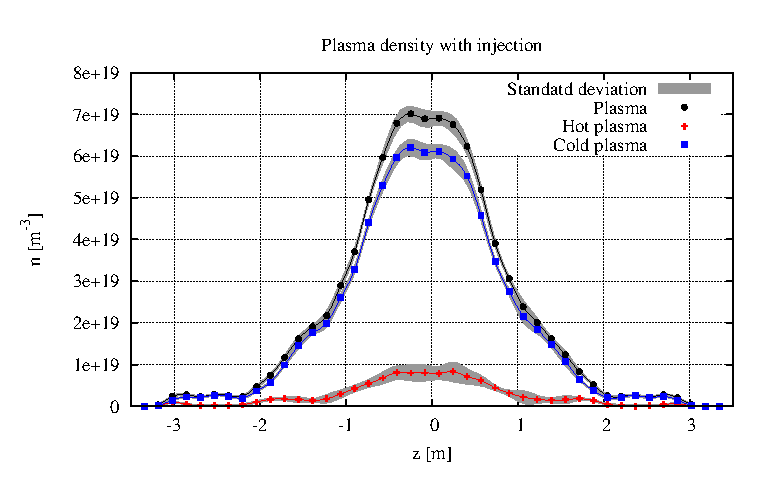
\includegraphics[width=1.\linewidth]{fig/ch5/dt11-with_sources/eps/density_z}
	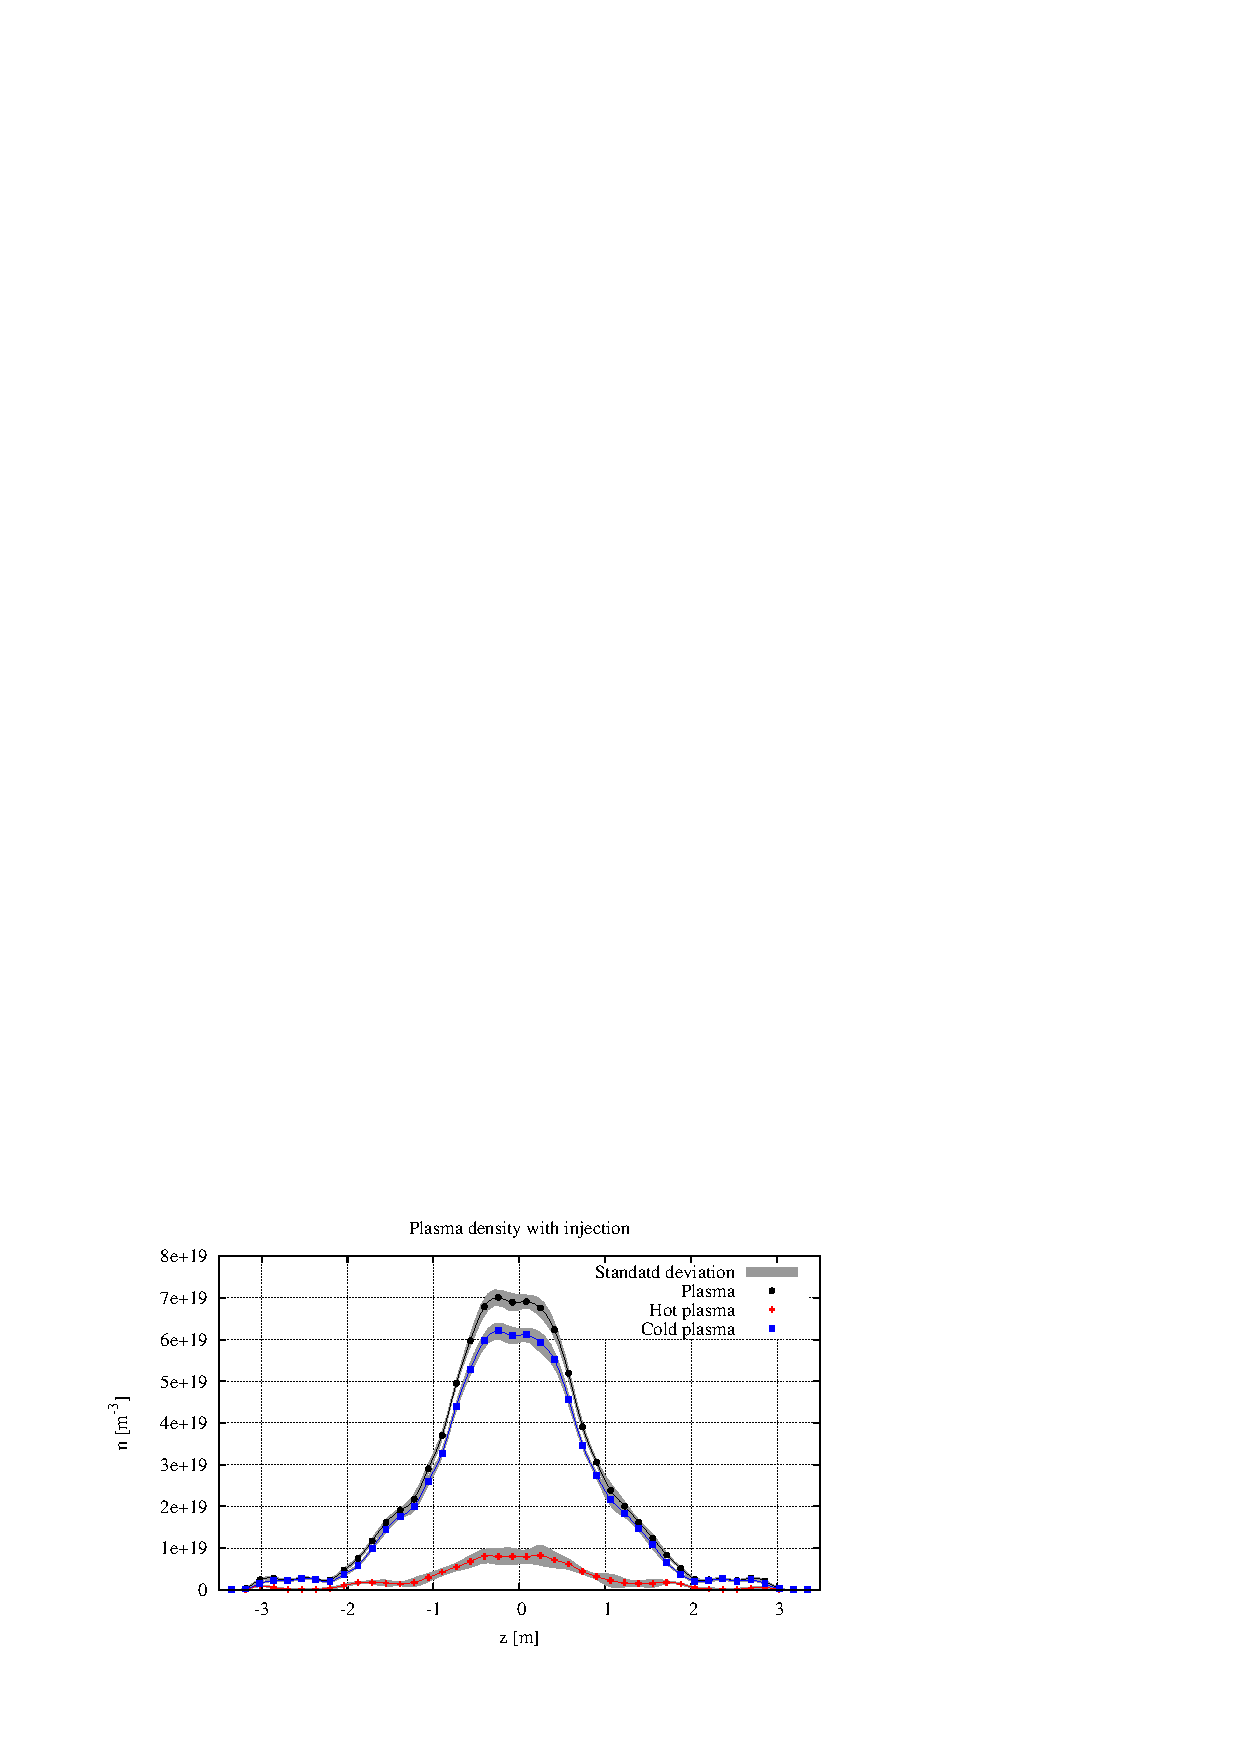
\includegraphics[width=1.\linewidth]{fig/ch5/density_z.png}
	\caption{Линейный профиль плотность плазмы при наличии инжекции}
	\label{fig:density_z}
\end{figure}

\subsection{Распределение температуры}

На графиках температуры уже явно видно, что при в областях с большей магнитной индукцией начинается расходимость. Также, анализируя графики а и б на рисунке \ref{fig:temperature}, необходимо принимать во внимание графики плотностей на рис. \ref{fig:density_r} и рис. \ref{fig:density_z} соответственно.

Проанализировав графики, можно сделать вывод о том, что температура слабо зависит от расстояния до оси симметрии. Однако, данный вывод расходится с экспериментальными наблюдениями --- температура, хоть и слабо, но убывает с увеличением расстояния до оси симметрии.

\begin{figure}[h!]
	\begin{minipage}[h]{0.89\linewidth}
		\center{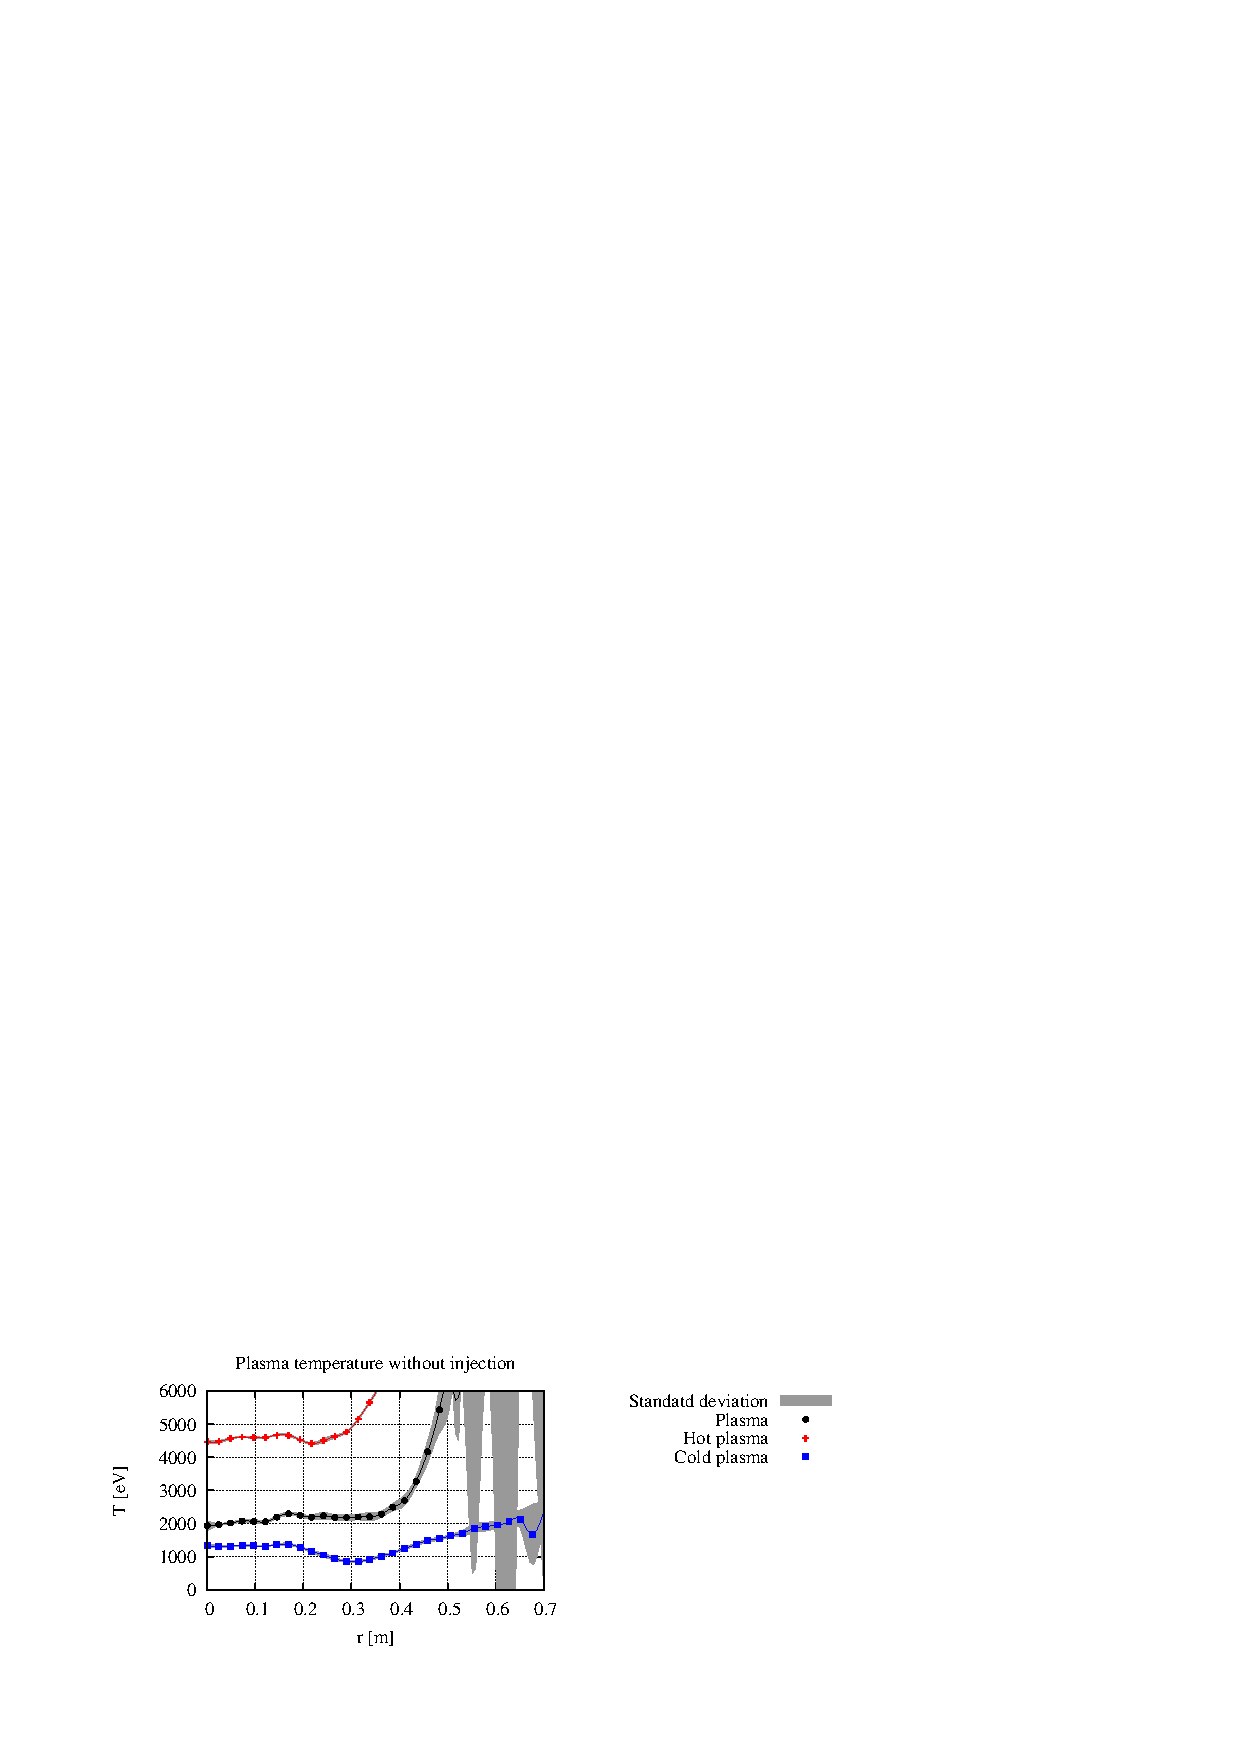
\includegraphics[width=1.1\linewidth]{fig/ch5/temperature_r.png} \\ \qquad \qquad а) }
	\end{minipage}
	\hfill
	\begin{minipage}[h]{0.89\linewidth}
		\center{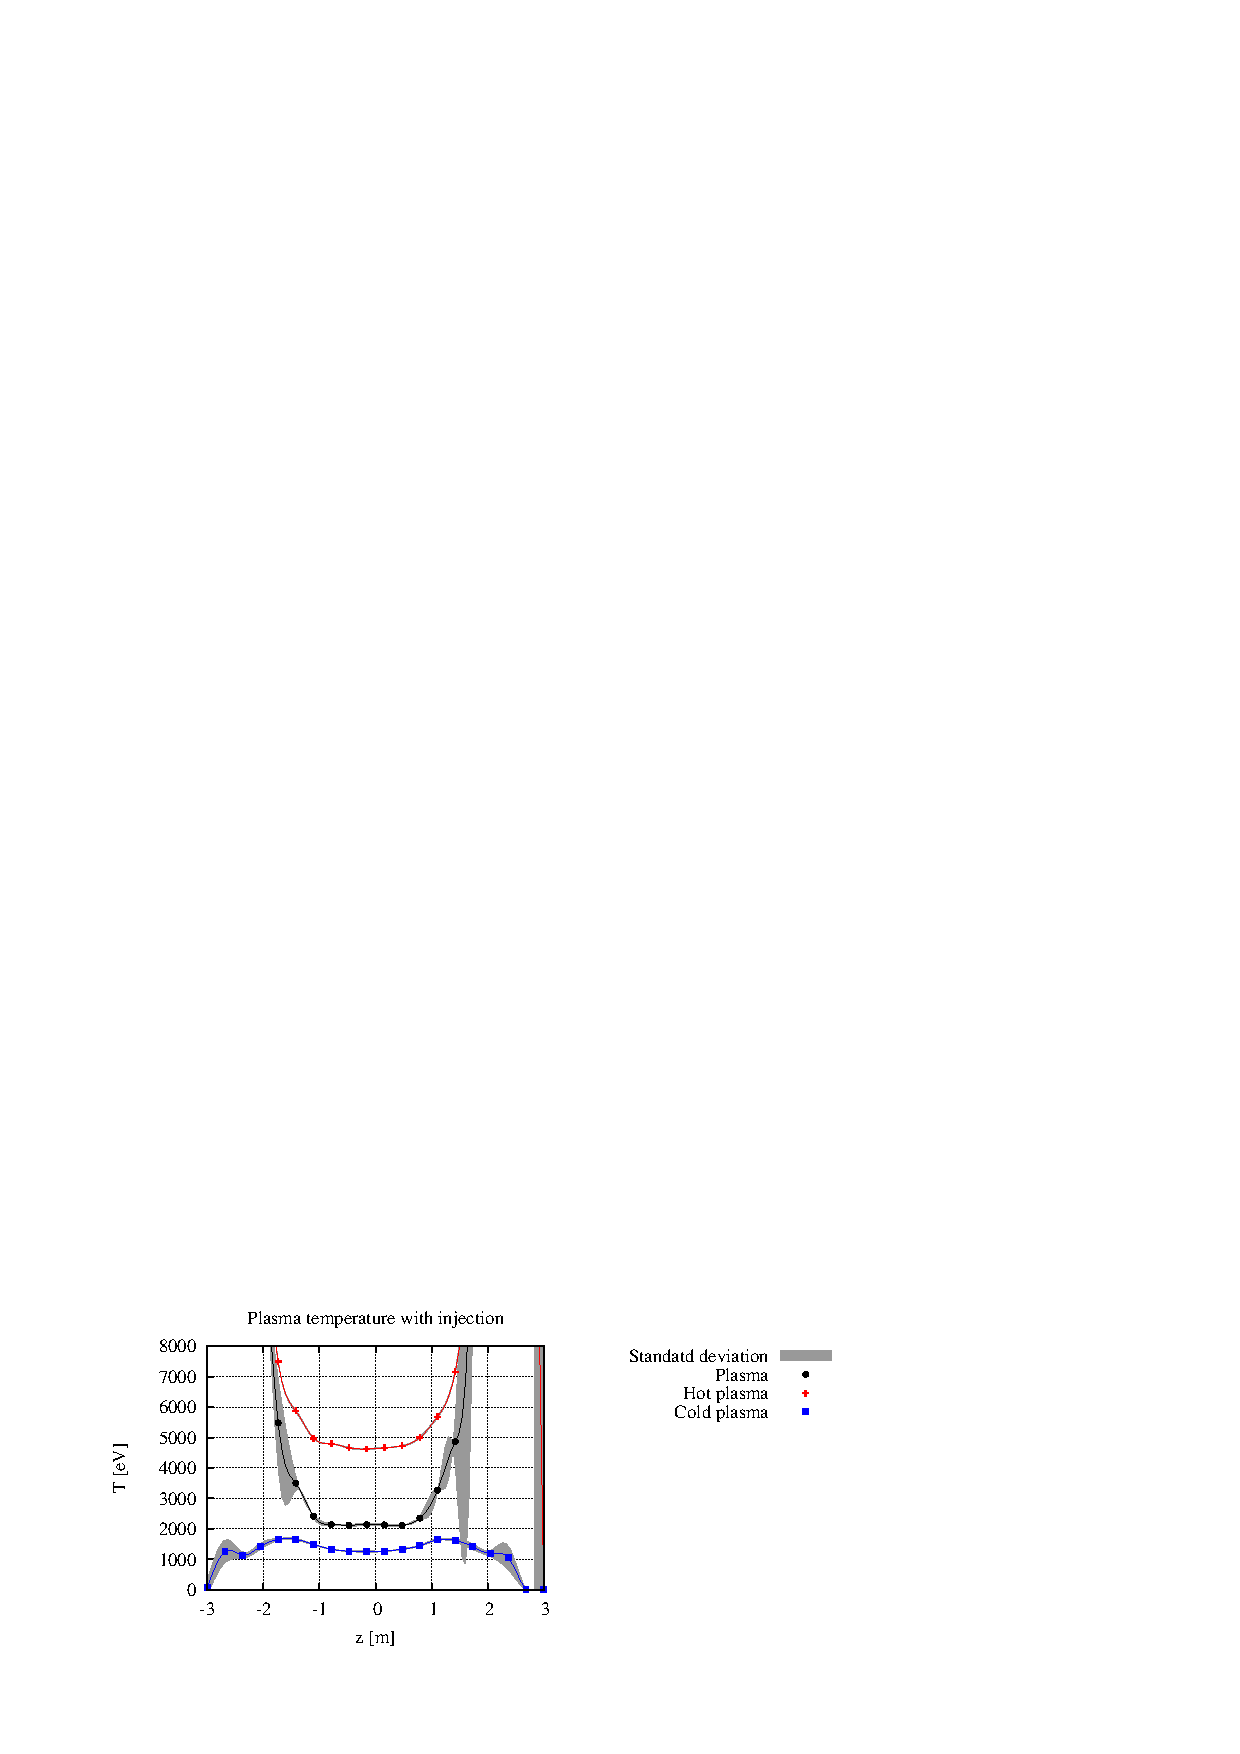
\includegraphics[width=1.1\linewidth]{fig/ch5/temperature_z.png} \\ \qquad \qquad б)}
	\end{minipage}
	\caption{Распределение температуры плазмы в установке: а) радиальное распределение; б) линейное распределение}
	\label{fig:temperature}
\end{figure}

\subsection{Распределение по скоростям}

Распределение по скоростям всегда получалось Максвелловским с хорошей степенью точности (типичная график представлен на рисунке \ref{fig:maxwell}). Причём никаких значительных отклонений в зависимости от места измерения тоже не было обнаружено.

\begin{figure}[h!]
	\centering
	\includegraphics[width=0.75\linewidth]{fig/ch5/maxwell}
	\caption{Распределение ионов по скоростям}
	\label{fig:maxwell}
\end{figure}


\subsection{Сравнение экспериментов с инжекцией и без инжекции горячих ионов}

Ощутимая разница наблюдается только на графиках радиальной плотности (рисунок \ref{fig:density_r_w}). Без инжекции провал становится более плавный и без дополнительного локального минимума.

\begin{figure}[h!]
	\center
	\includegraphics[width=1.\linewidth]{fig/ch5/density_comp}
	\caption{Радиальный профиль плотность плазмы при наличии и отсутствии инжекции}
	\label{fig:density_r_w}
\end{figure}

\section{Перспективы развития модели}

Построенная модель учитывает не все явления. Логическим продолжением развития данного исследования может стать добавление учёта процессов ионизации и реакций термоядерного синтеза. Создание гибридной модели, учитывающей как движение электронов, так и движение ионов, причём делать это пошагово --- при движении электронов считать ионы неподвижными, а при расчёте ионов добавлять экранирующую функцию. Каждый шаг возможно будет связать с предыдущим рассчитанными распределением потенциала. Кроме того, необходимо учесть влияние металлических стенок конструкции, а также множество дополнительно установленных систем стабилизации, например созданное радиальное электрическое поле для подавление МГД неустойчивости и уменьшения радиальных потерь.

Также с помощью полученных данных, возможно уже получить начальные распределения $n(\vec{r})$ для более сложных вычислений.	       % Глава 4 -- числ. эксп



\chapter*{ЗАКЛЮЧЕНИЕ}						% Заголовок
\addcontentsline{toc}{chapter}{ЗАКЛЮЧЕНИЕ}	% Добавляем его в оглавление

%% Согласно ГОСТ Р 7.0.11-2011:
%% 5.3.3 В заключении диссертации излагают итоги выполненного исследования, рекомендации, перспективы дальнейшей разработки темы.
%% 9.2.3 В заключении автореферата диссертации излагают итоги данного исследования, рекомендации и перспективы дальнейшей разработки темы.
%% Поэтому имеет смысл сделать эту часть общей и загрузить из одного файла в автореферат и в диссертацию:

В процессе выполнения работы был произведён обзор современных установок по удержанию субтермоядерной плазмы, а также обзор численных методов, применяемых для описания подобных систем. Было выяснено, что есть возможность применения метода молекулярной динамики при решении задач больш\'{о}го масштаба.

Основные результаты работы заключаются в следующем:
%% Согласно ГОСТ Р 7.0.11-2011:
%% 5.3.3 В заключении диссертации излагают итоги выполненного исследования, рекомендации, перспективы дальнейшей разработки темы.
%% 9.2.3 В заключении автореферата диссертации излагают итоги данного исследования, рекомендации и перспективы дальнейшей разработки темы.
\begin{enumerate}
  \item Для выполнения поставленных задач был создан ряд многоцелевых вычислительных программ, написанных на языках \texttt{c++} и Python.
  \item Получена конфигурация магнитного поля открытой ловушки аналогичной используемой в ГДЛ.
  \item В результате проведения серии численных экспериментов по моделированию поведения горячей плазмы в открытой магнитной ловушке получен набор параметров (плотность, температура, распределение по скоростям), характеризующих динамику горячих ионов.
  \item Сопоставление результатов численных экспериментов с экспериментальными данными позволяет сделать вывод о применимости составленной модели в задачах, где требуется оценочные результаты. Модель позволяет качественно правильно рассчитать распределение концентрации в объёме установки, а также распределение частиц по скоростям.
\end{enumerate}


Развив данную модель, а именно добавив учёт процессов ионизации, термоядерных реакций, более точный расчёт внешнего электромагнитного поля (в том числе учесть дополнительные системы стабилизации), станет возможным исследовать более тонкие эффекты. Результаты данной работы могут служить отправной точкой в следующем этапе исследований.
      % Заключение


\include{Dissertation/references}      % Список литературы
%\include{Dissertation/lists}           % Списки таблиц и изображений (иллюстративный материал)
%\input{Dissertation/appendixsetup}   % Предварительные настройки для правильного подключения Приложений

\chapter{Аналитическое решение уравнения движения одиночного электрона} \label{AppendixA}


%Листинг~\ref{list:external1} подгружается из внешнего файла. Приходится загружать без окружения дополнительного. Иначе по страницам не переносится.
%\lstinputlisting[lastline=78,language={R},caption={Листинг из внешнего файла},label={list:external1}]{listings/run_analysis.R}


        % Приложения

\end{document}
